

%This method is Monte-Carlo based, and makes use of the samples corresponding to the various processes expected to produce fake leptons. 
%Correction factors of the fake lepton modeling in the simulation are determined 
%in a combined fit of several control regions involving shapes of discriminant variables such as the missing transverse momentum or the jet multiplicity. 
%There are five such correction factors (for fake electrons and muons originating from light or heavy flavor jets, and an additional factor for charge flip), 
%which are applied on an event basis depending on the generator information about the origin of the fake lepton in the event. 
%More details can be found in the documentation of the Run-1 analysis~\cite{noteSS3L}. 

% for now I am including everything in this section, later i can put details in an appendix.
% Additional information regarding the method is presented in Appendix ??.

We describe in this section a simulation-based method that provides an alternative estimate of the data-driven backgrounds in the signal regions. 
The method is based on different assumptions than the matrix method described in Section~\ref{sec:bkg_matrix_method}, 
and is intended primarily as a cross-check. 
We provide here a brief description of the MC method and present its background predictions for the signal regions. More details about the method can be found in Appendix \ref{app_mc_template}.

The MC-based method relies on MC simulations to extrapolate background predictions from control regions with low \met , \meff , 
and jet multiplicity to the signal regions (where \met , \meff , or jet multiplicity are required to be high). 
The control regions are used to rescale MC samples with ``fake'' leptons so that they match the observed data. 
The main assumption of the method is that the MC simulations describe the kinematic distributions correctly (within the limited MC precision) 
and predict accurately the rate of fake leptons up to a global factor (for each type of fake lepton) independent of the event kinematics and the process type. 
This assumption makes the method a suitable cross-check of the matrix method, that assumes that the lepton fake rates 
are the same in control and signal regions regardless of the selection requirements. 
The other assumption is that the fake rates are uncorrelated in events with multiple fake leptons.
Six non-overlapping control regions are defined by presence of $b$-jets and the flavors of the same sign leptons in the event:

\begin{itemize}
\item CR0b: events without $b$-jets where the leptons are $ee$, $e\mu$, and $\mu\mu$.
\item CR1b: events with at least one $b$-jet where the leptons are $ee$, $e\mu$, and $\mu\mu$.
\end{itemize}

All the selected events contain two same-sign or more signal leptons and \met >25 GeV. 
Events satisfying the signal regions requirements are excluded from the control regions. 
The purpose of the \met requirement is to remove multi-jet events that have two or more ``fake'' leptons and tend to have low \met. 

The next step is to classify events into separate categories depending on the lepton source process. 
The three main categories are prompt isolated leptons, charge flip electrons, 
and ``fake'' leptons which consist of non-prompt leptons coming from hadron decays and hadrons misidentified as leptons. 
The fakes are further separated by lepton flavor and the jet flavor producing the fake lepton. 
The last separation is due to $b$-tagging where a $b$-tagged sample will be enhanced in $b$-quark induced fakes. 
To make the $b$-tagging requirement orthogonal to the fake rate correction, we separate the leptons that are coming from $b$-hadron decays, 
labelled as heavy-flavor (HF), from the rest of the fakes, labelled as light-flavor (LF), and derive a fake rate correction for each category.
The classification is done based on the parent particle from the generator event record using the type and origin of the lepton provided by the MCTruthClassifier.

In total we have five categories (charge flip, EL HF, MU HF, EL LF, MU LF) that we derive correction factors for using a simulatenous fit to data in six control regions (CR0b and CR1b for $ee$, $e\mu$, and $\mu\mu$ channels).
The fit uses a likelihood function defined as the product of the Poisson probabilities describing the observed events in the binned distributions from the expected number 
of events rescaled by the five correction factors which are left free in the fit.  
These correction factors are applied to the MC predictions in the signal regions to obtain an estimation of the fake and charge flip backgrounds. 

The six distributions are chosen for variables that provide the best separation between processes with prompt leptons and processes with fake leptons and charge flip and are shown in 
Figure \ref{f:fit_CR0b} and Figure \ref{f:fit_CR1b}. 

\begin{figure}[htb]
  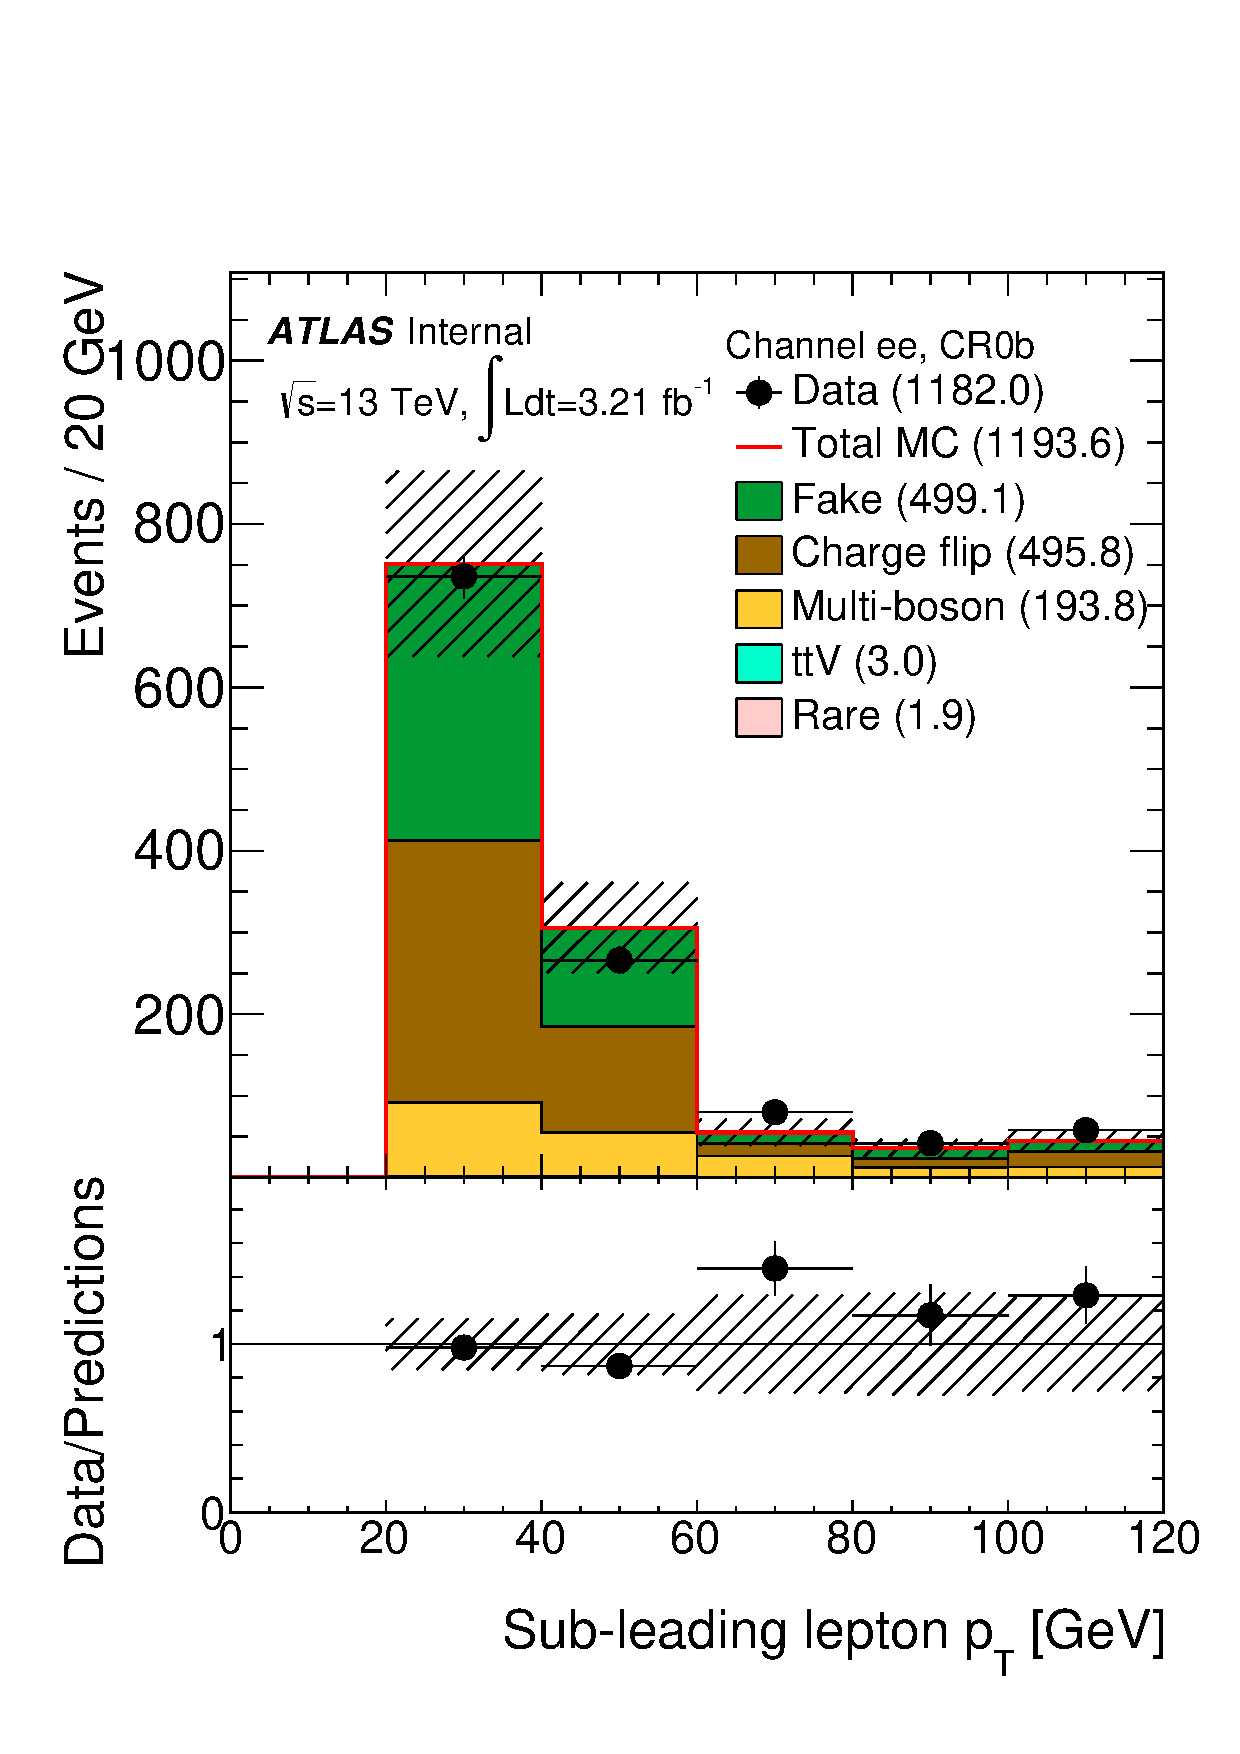
\includegraphics[width=.32\textwidth]{FIGURES/bckg_MC/SS3L/noFit/LEP2Pt_ee_CR0b_SS3L}
  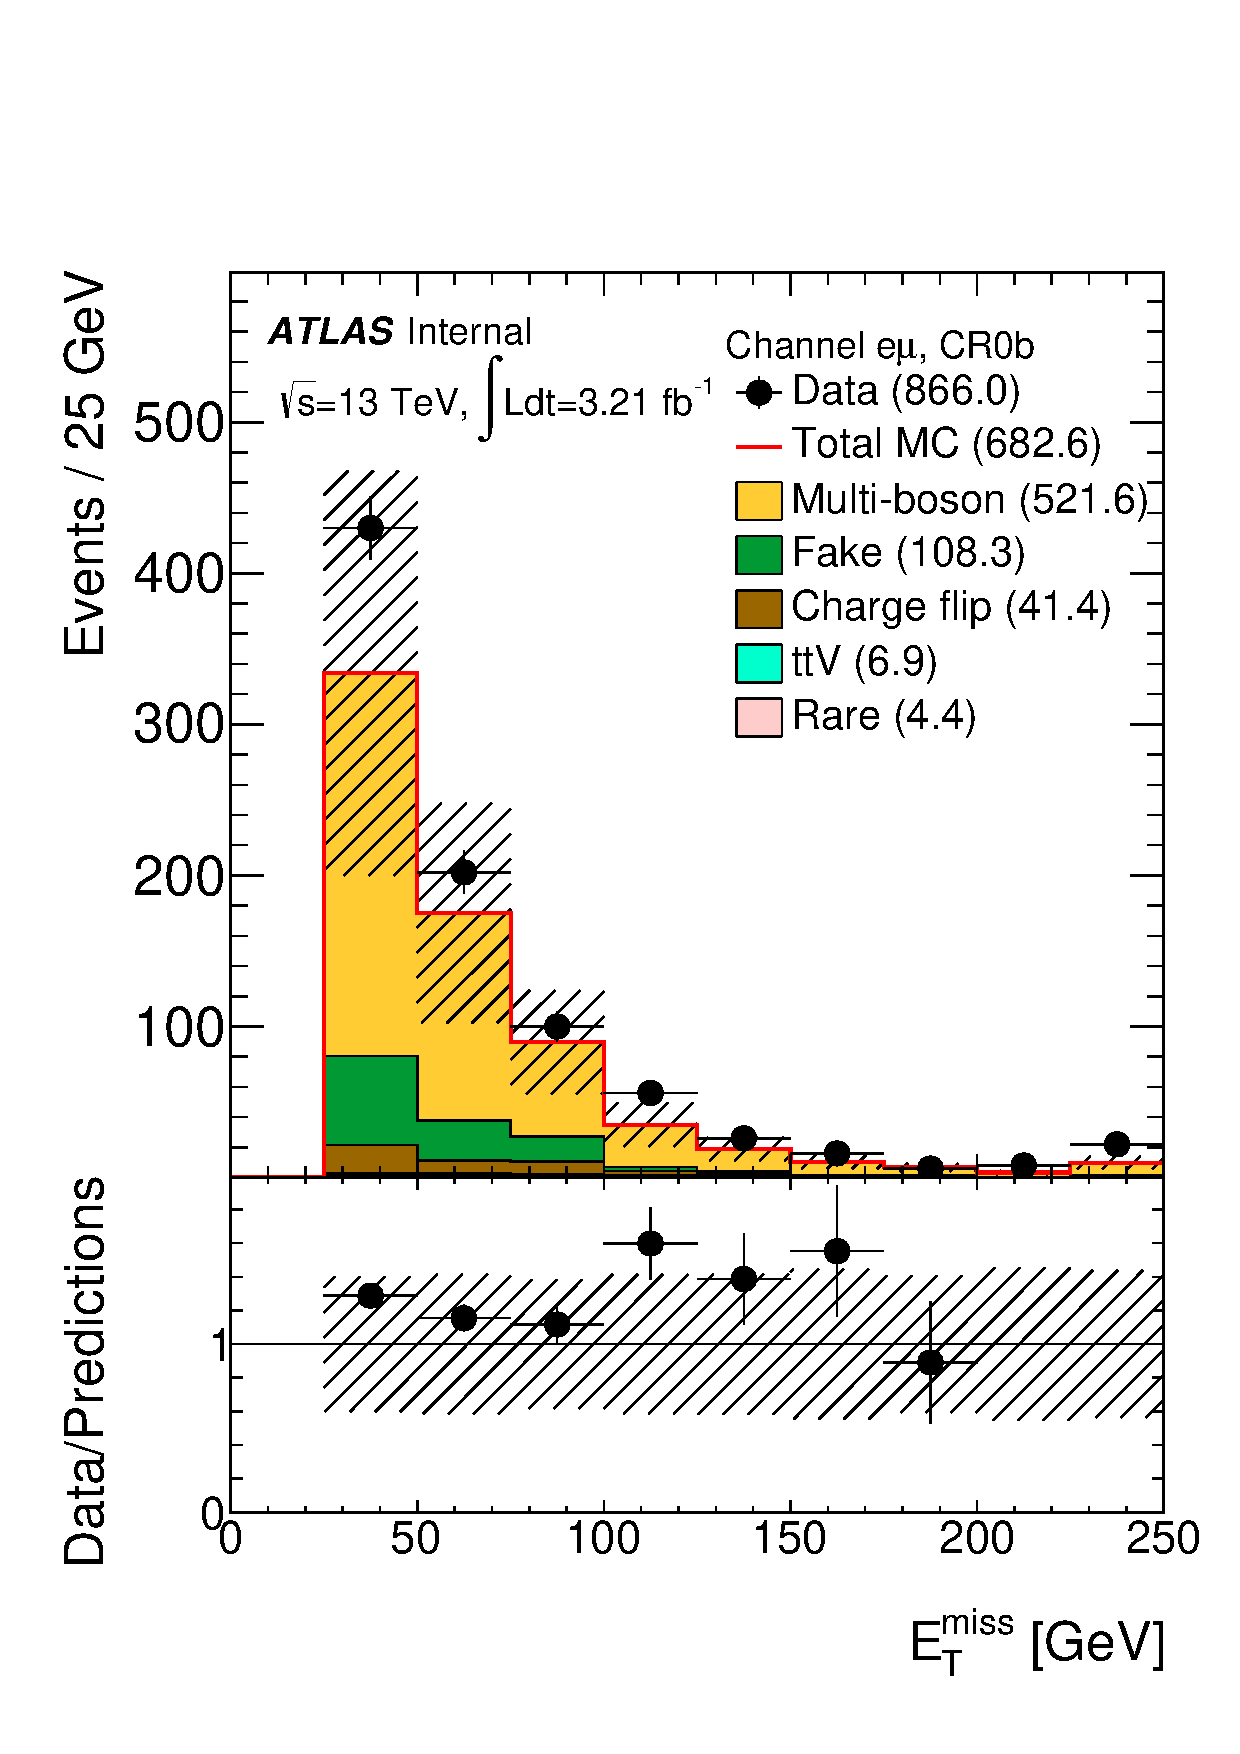
\includegraphics[width=.32\textwidth]{FIGURES/bckg_MC/SS3L/noFit/MET_em_CR0b_SS3L}
  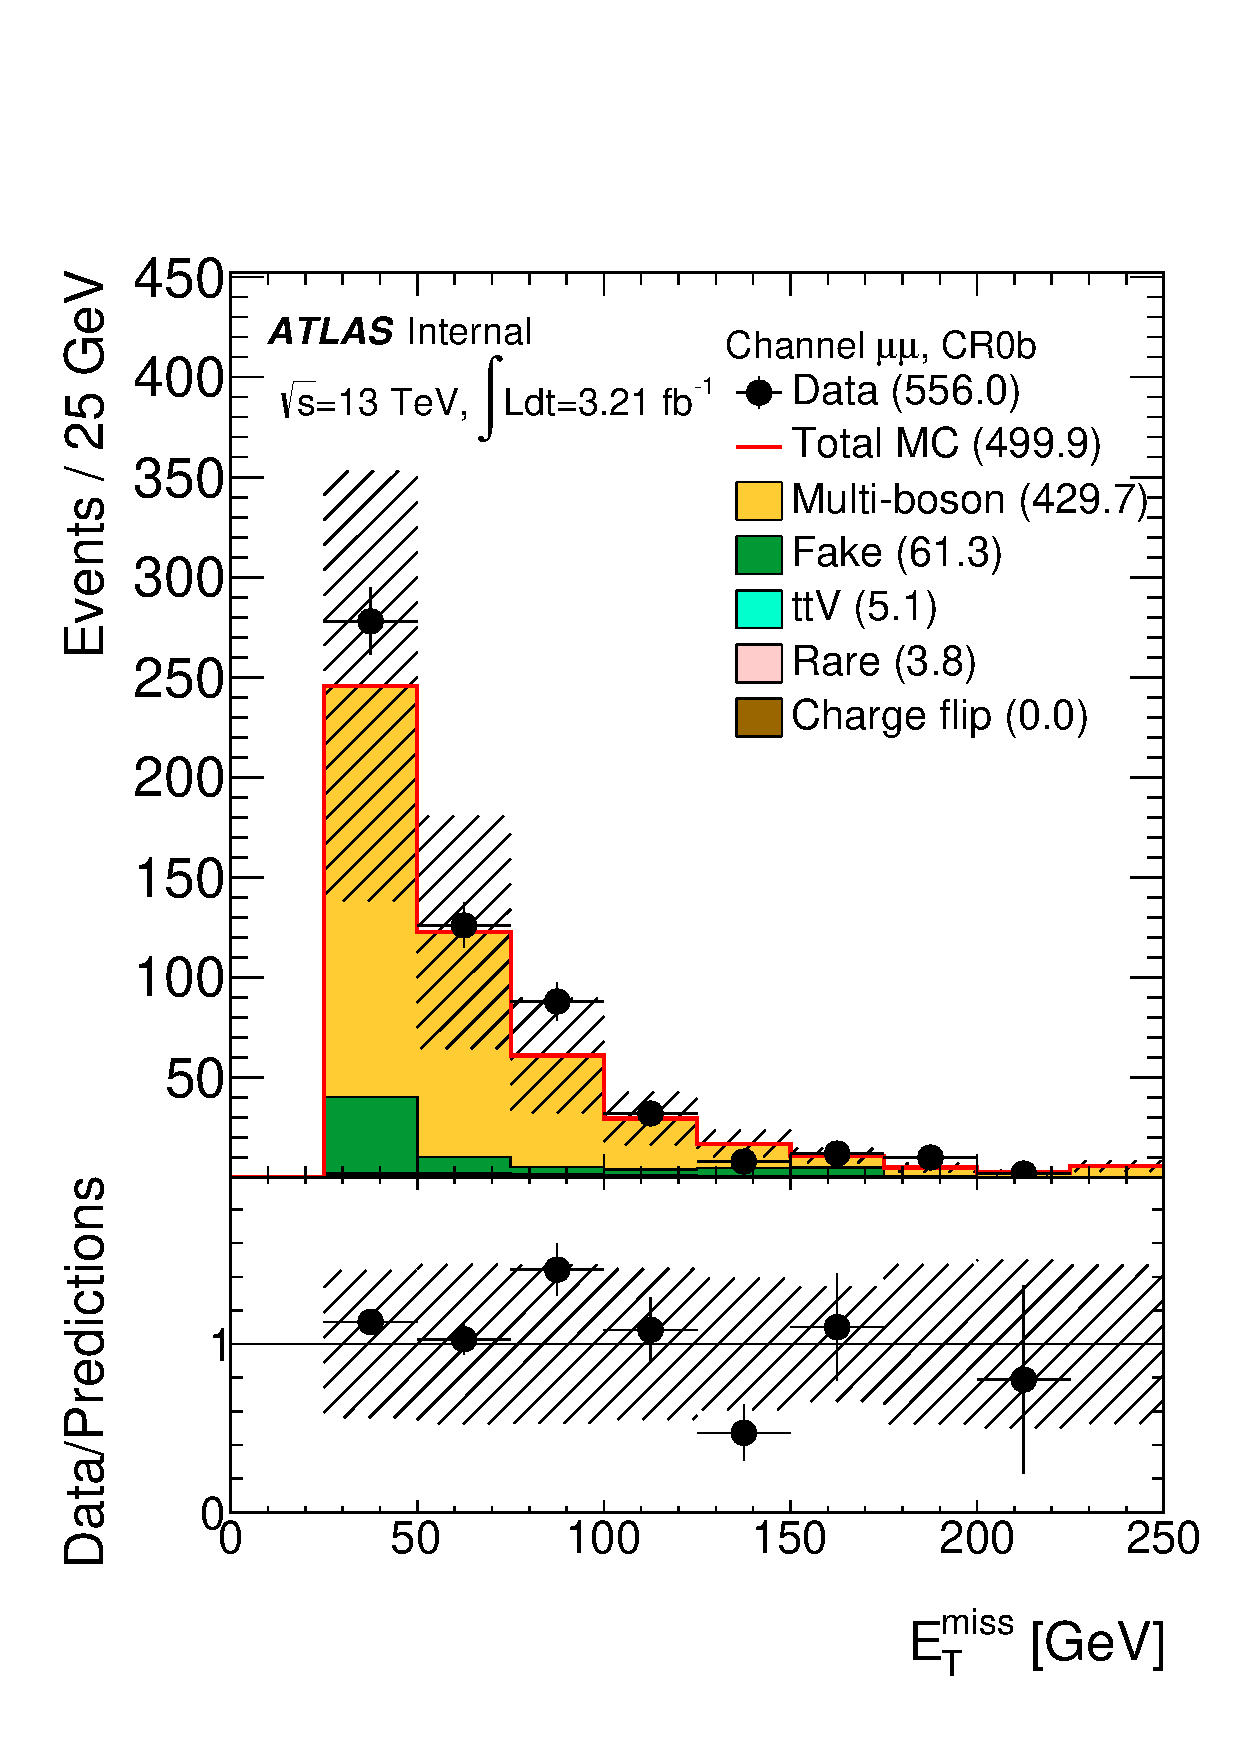
\includegraphics[width=.32\textwidth]{FIGURES/bckg_MC/SS3L/noFit/MET_mm_CR0b_SS3L}
\caption{
Pre-fit distributions for  $ee$ channel (left),  for  $e\mu$ channel (middle), and  for  $\mu\mu$ channel (right) from CR0b that were used in the fit to extract the fake rate and charge flip corrections.
 The hashed band represents the sum of systematic uncertainties on the predictions.
\label{f:fit_CR0b}
}
\end{figure}

\begin{figure}[htb]
  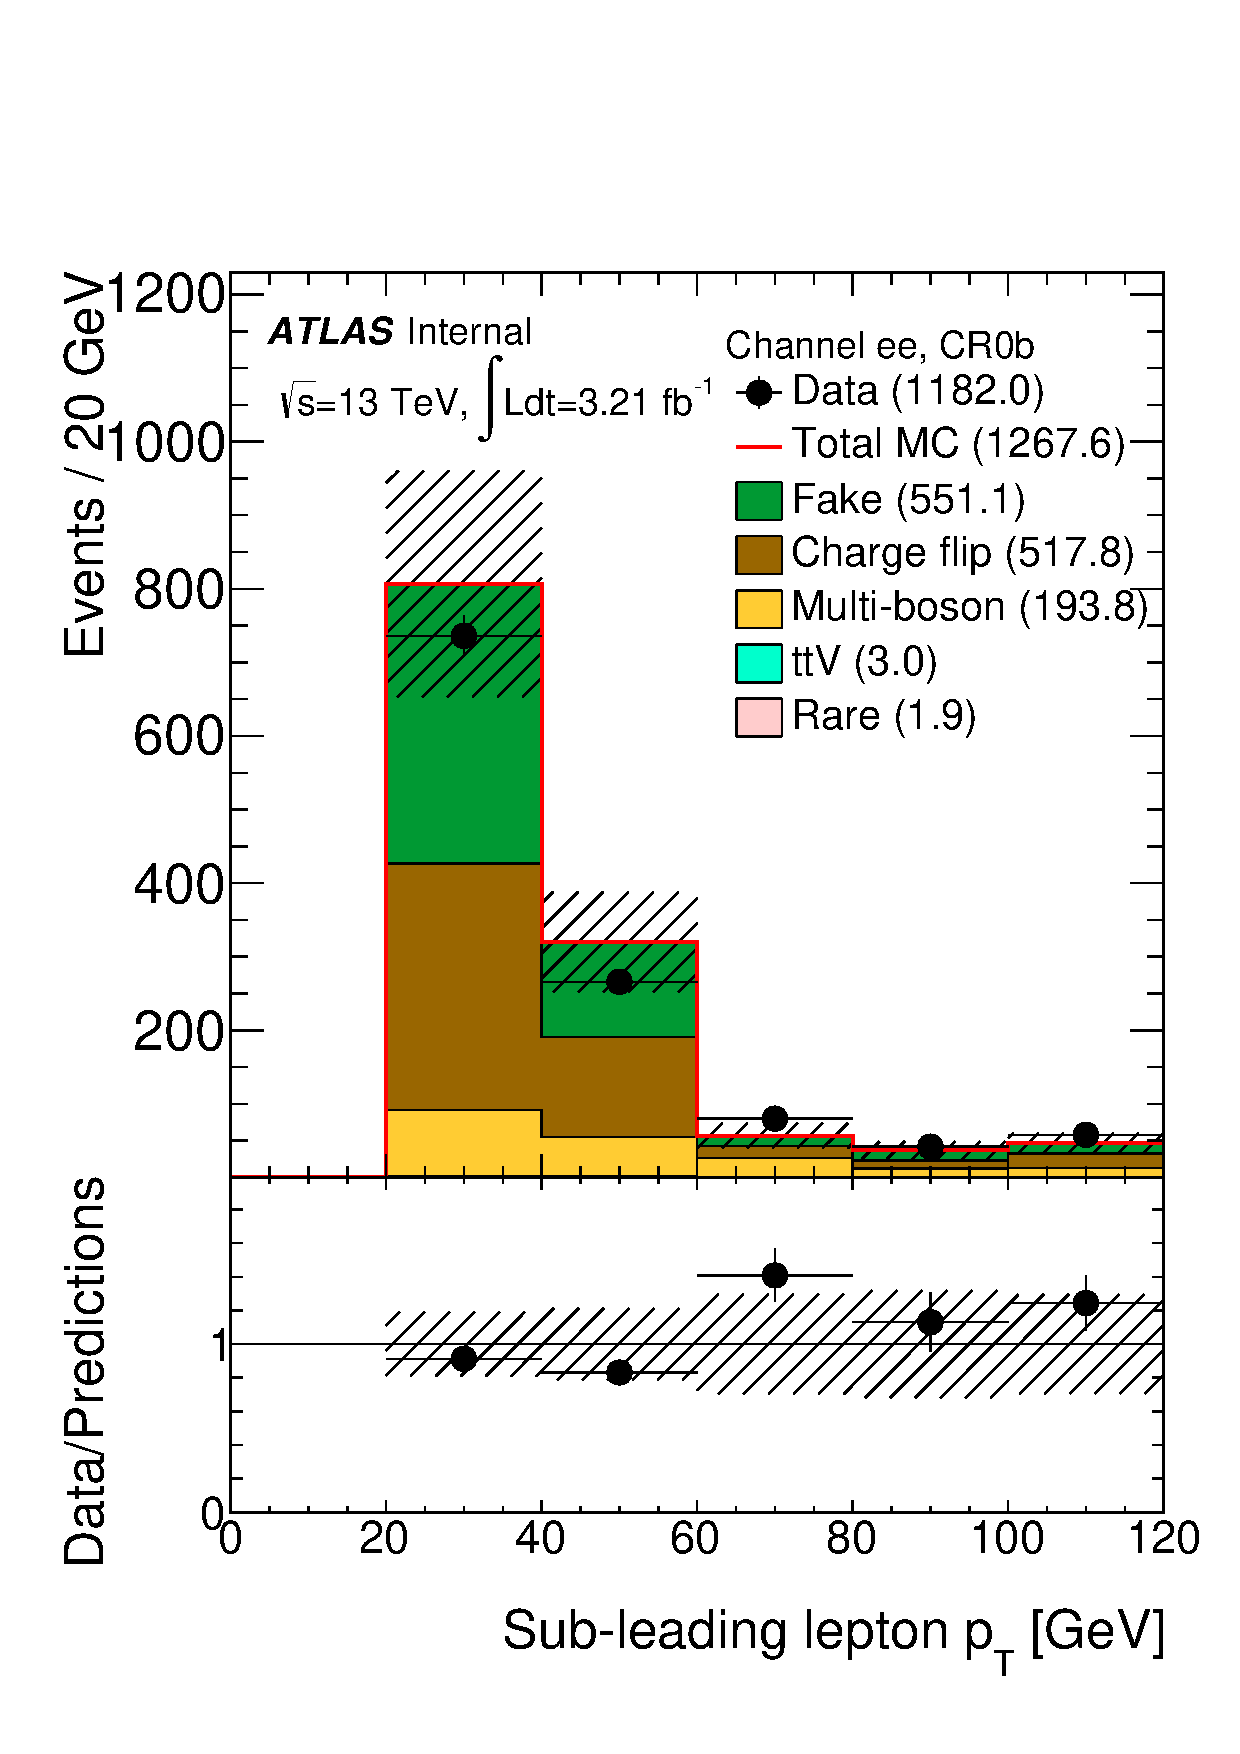
\includegraphics[width=.32\textwidth]{FIGURES/bckg_MC/SS3L/Fit/LEP2Pt_ee_CR0b_SS3L}
  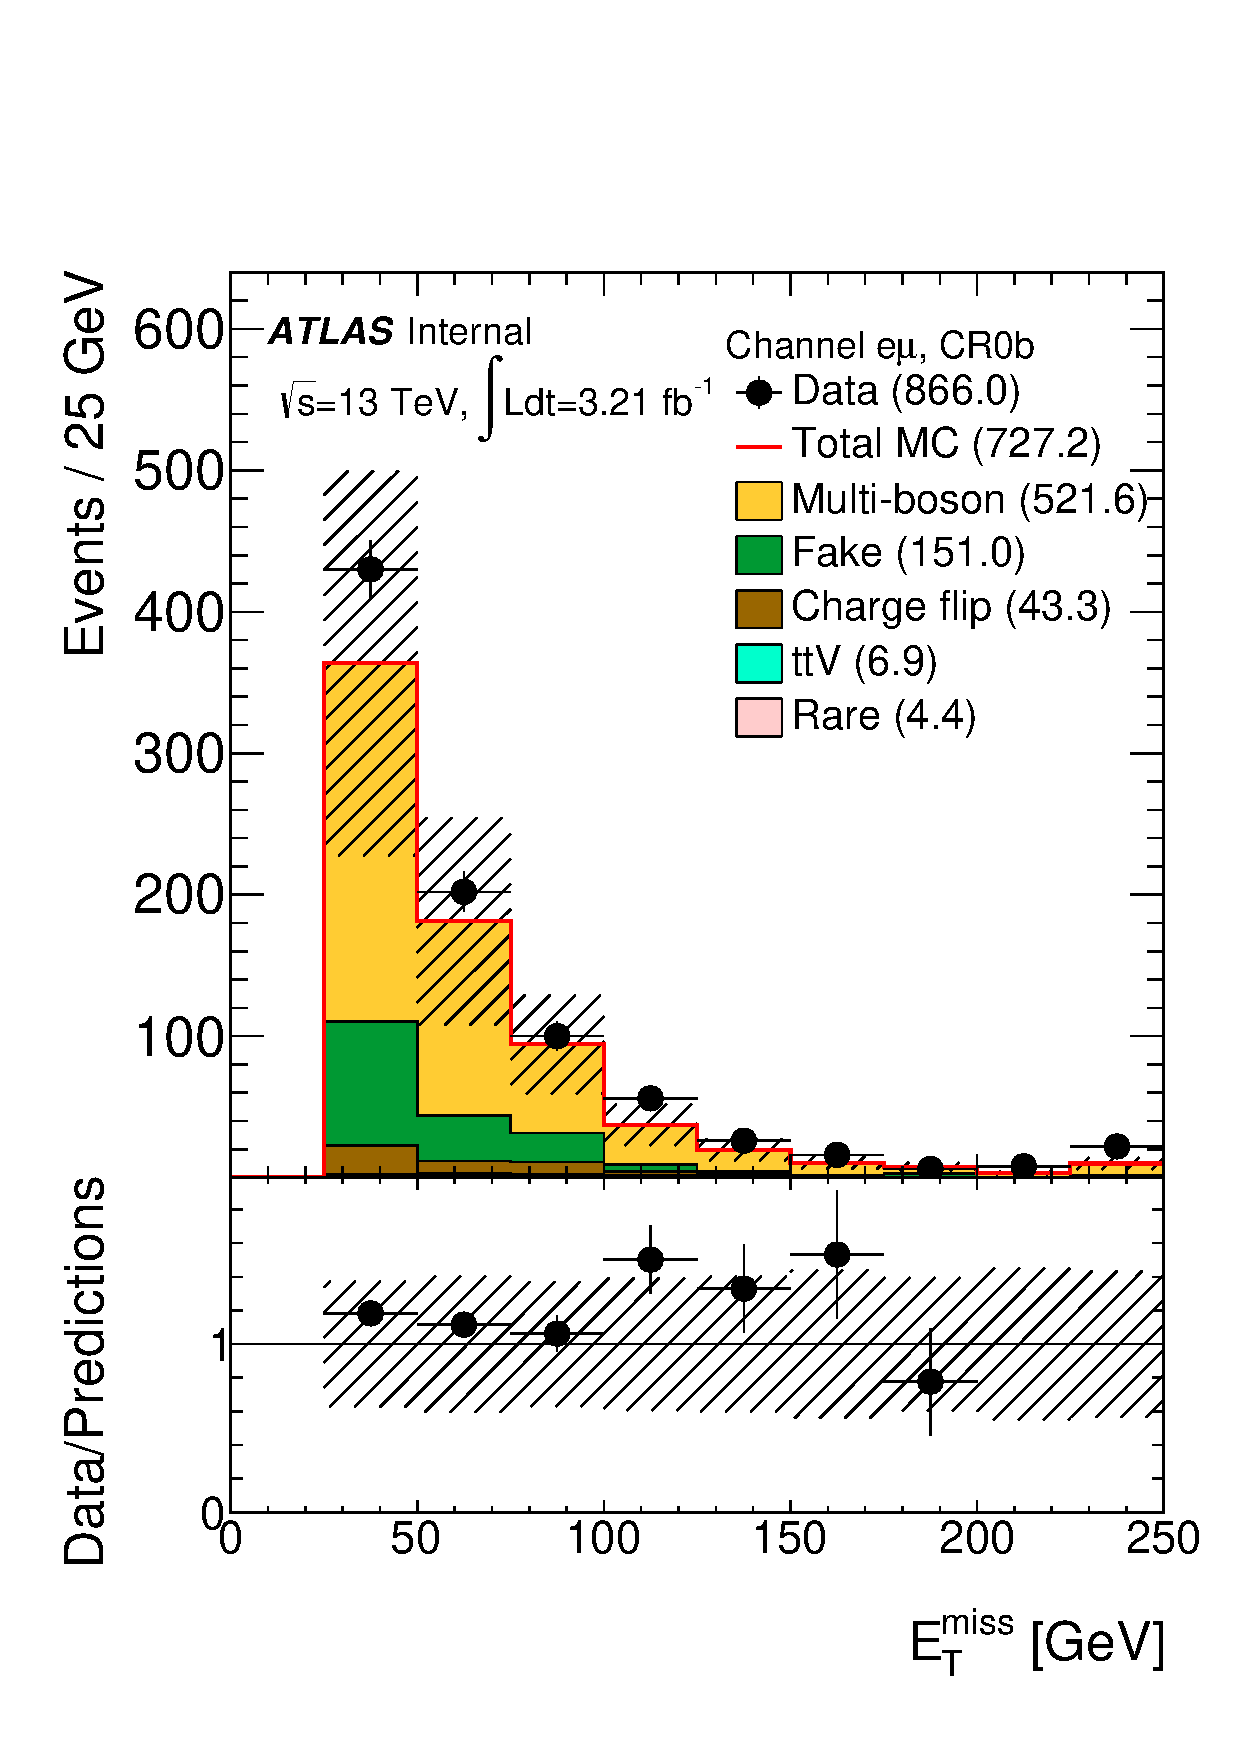
\includegraphics[width=.32\textwidth]{FIGURES/bckg_MC/SS3L/Fit/MET_em_CR0b_SS3L}
  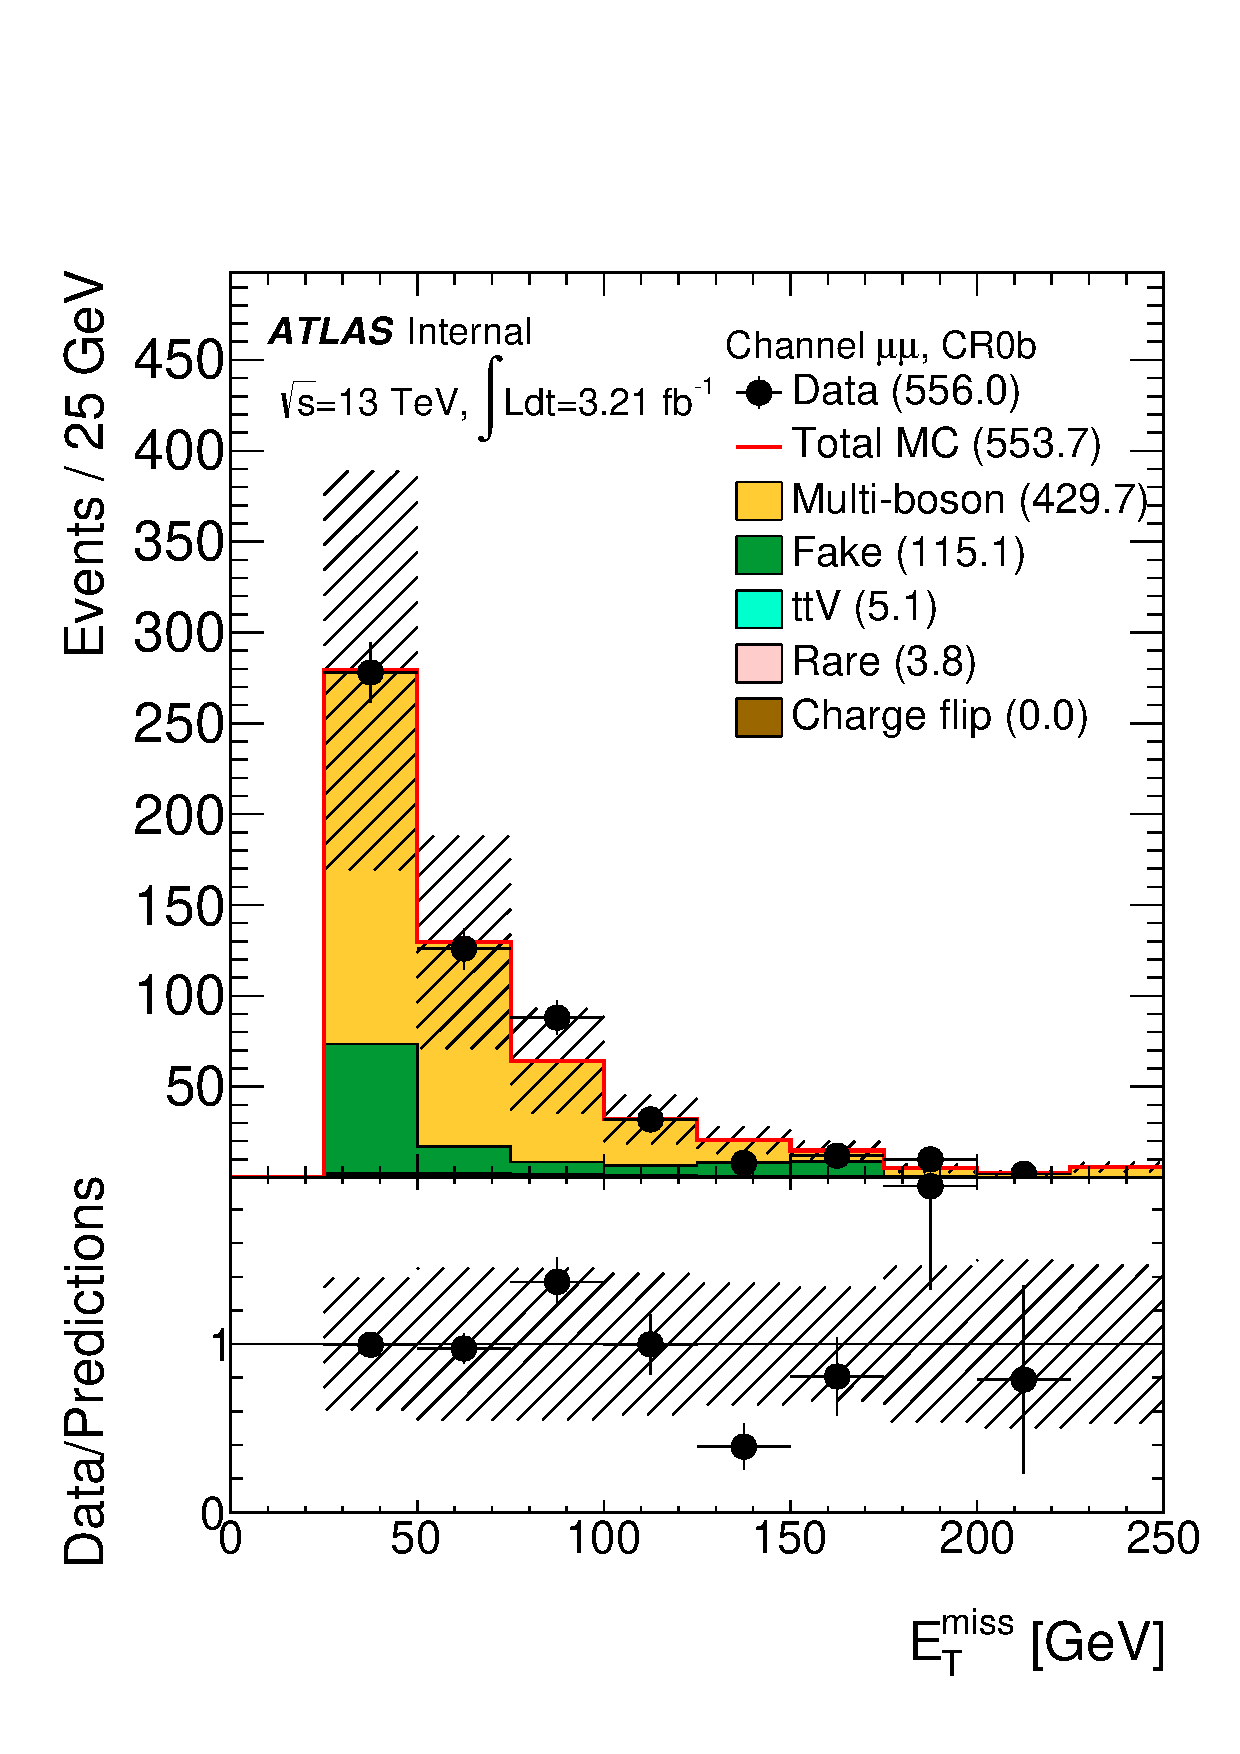
\includegraphics[width=.32\textwidth]{FIGURES/bckg_MC/SS3L/Fit/MET_mm_CR0b_SS3L}
\caption{
Post-fit distributions for  $ee$ channel (left),  for  $e\mu$ channel (middle), and  for  $\mu\mu$ channel (right) from CR0b that were used in the fit to extract the fake rate and charge flip corrections.
 The hashed band represents the sum of systematic uncertainties on the predictions.
\label{f:fit_CR0b}
}
\end{figure}

\begin{figure}[htb]
  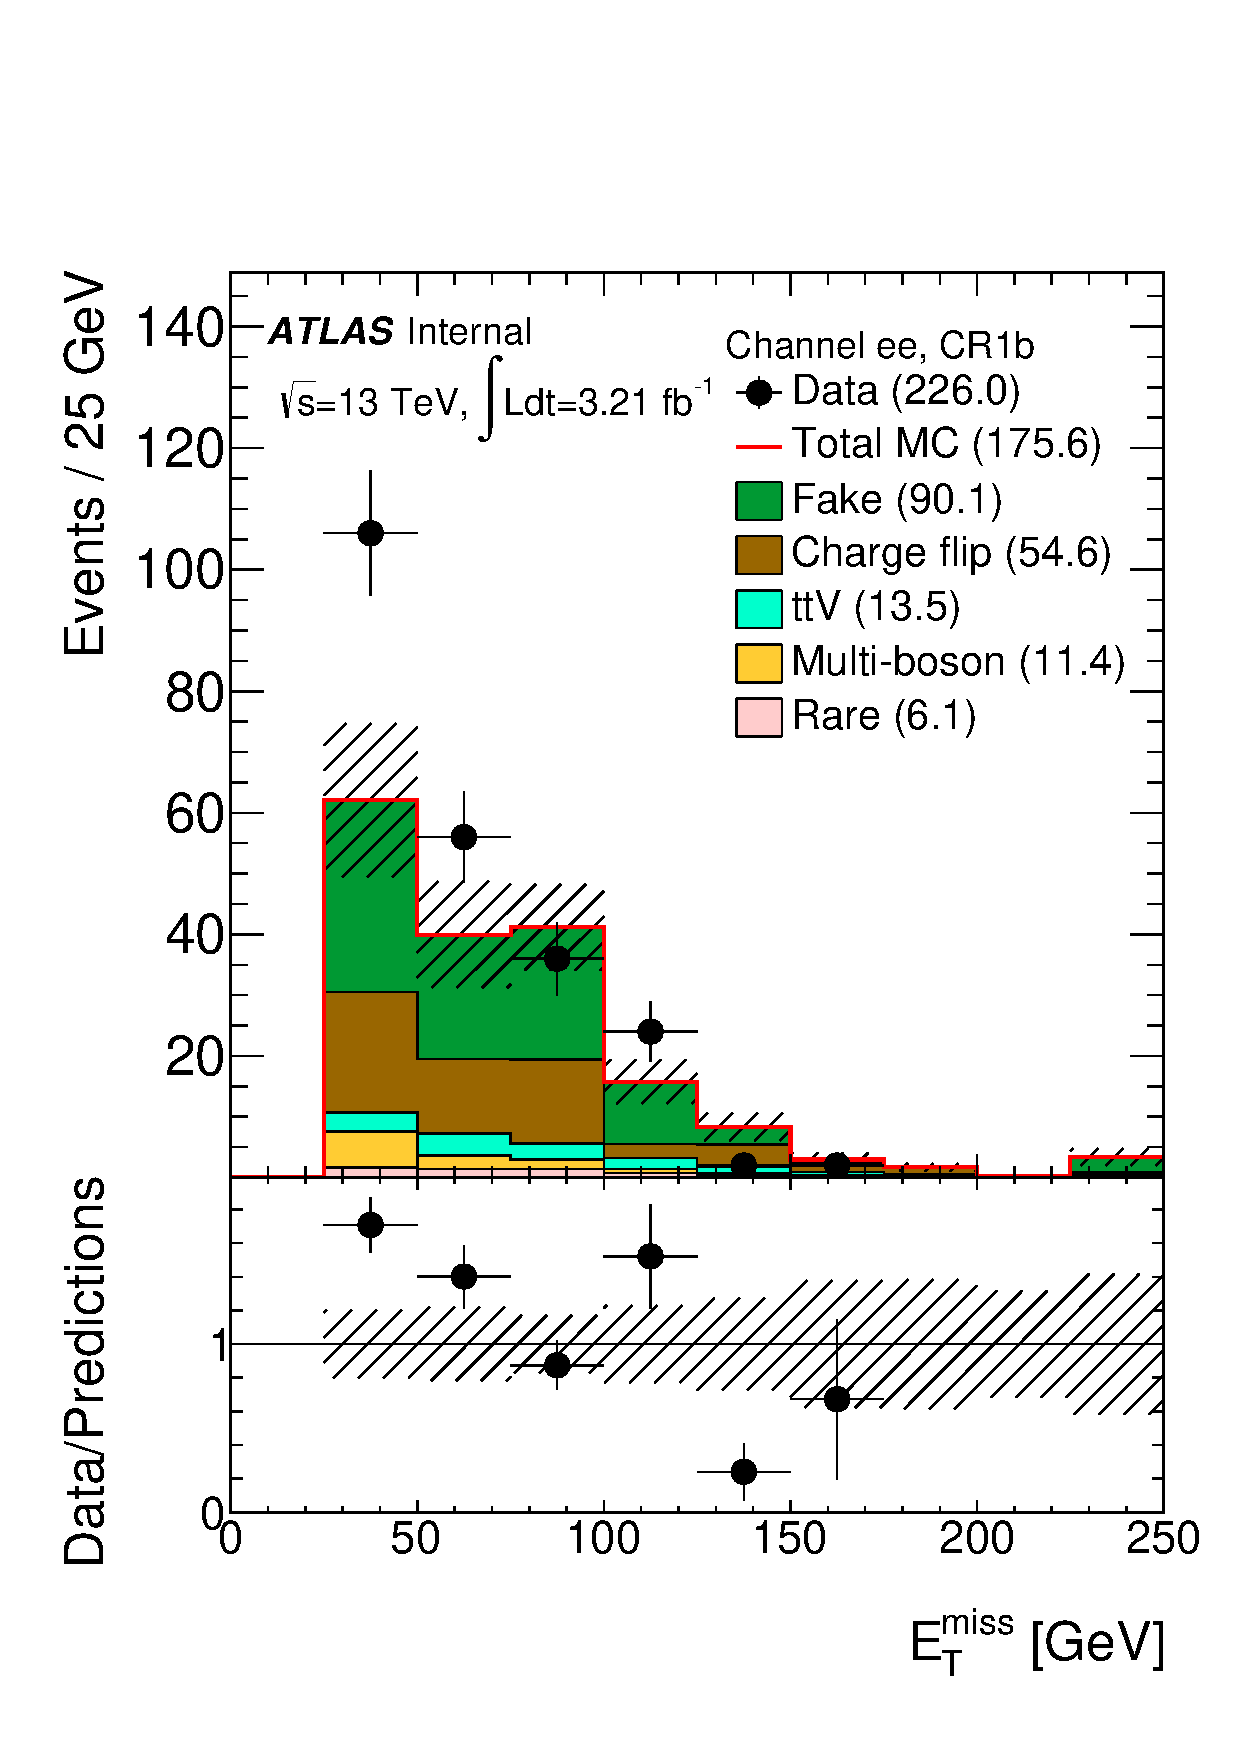
\includegraphics[width=.32\textwidth]{FIGURES/bckg_MC/SS3L/noFit/MET_ee_CR1b_SS3L}
  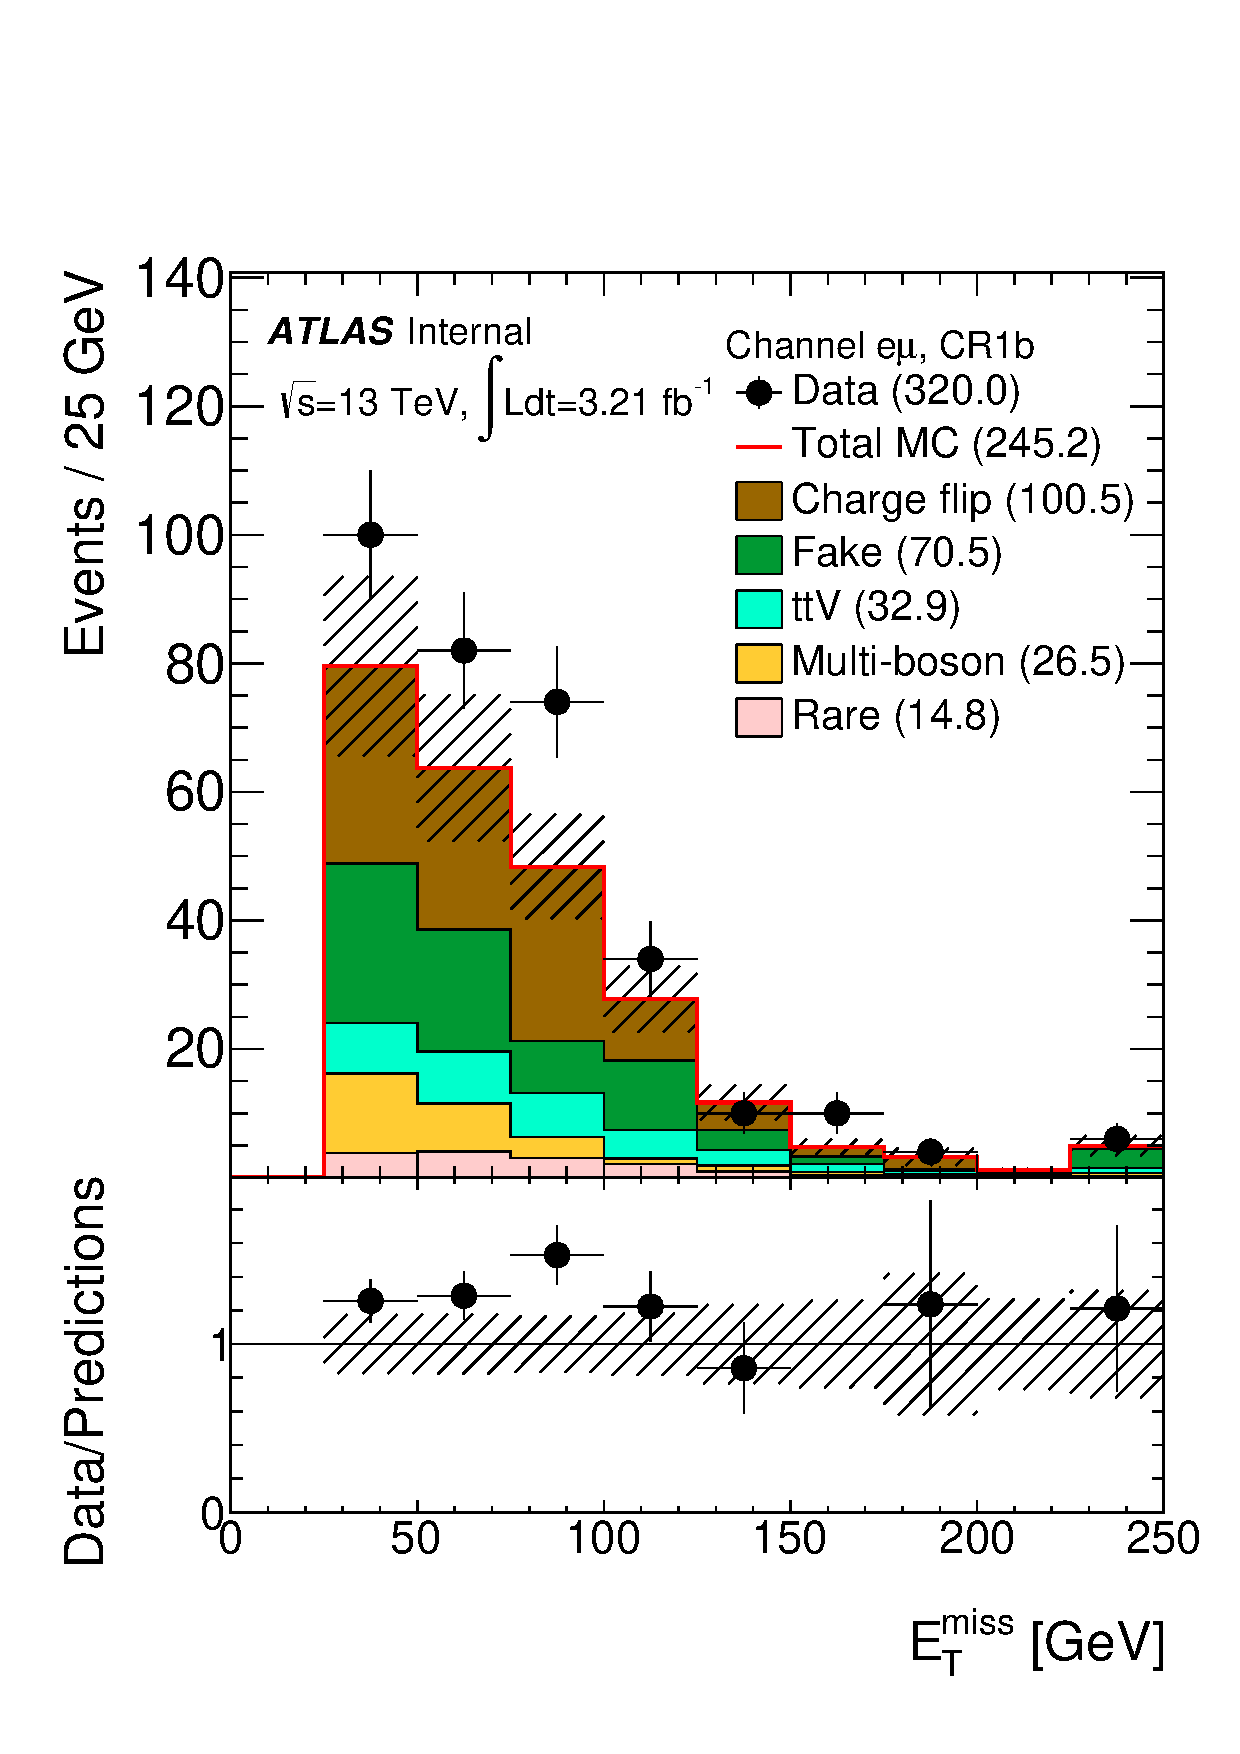
\includegraphics[width=.32\textwidth]{FIGURES/bckg_MC/SS3L/noFit/MET_em_CR1b_SS3L}
  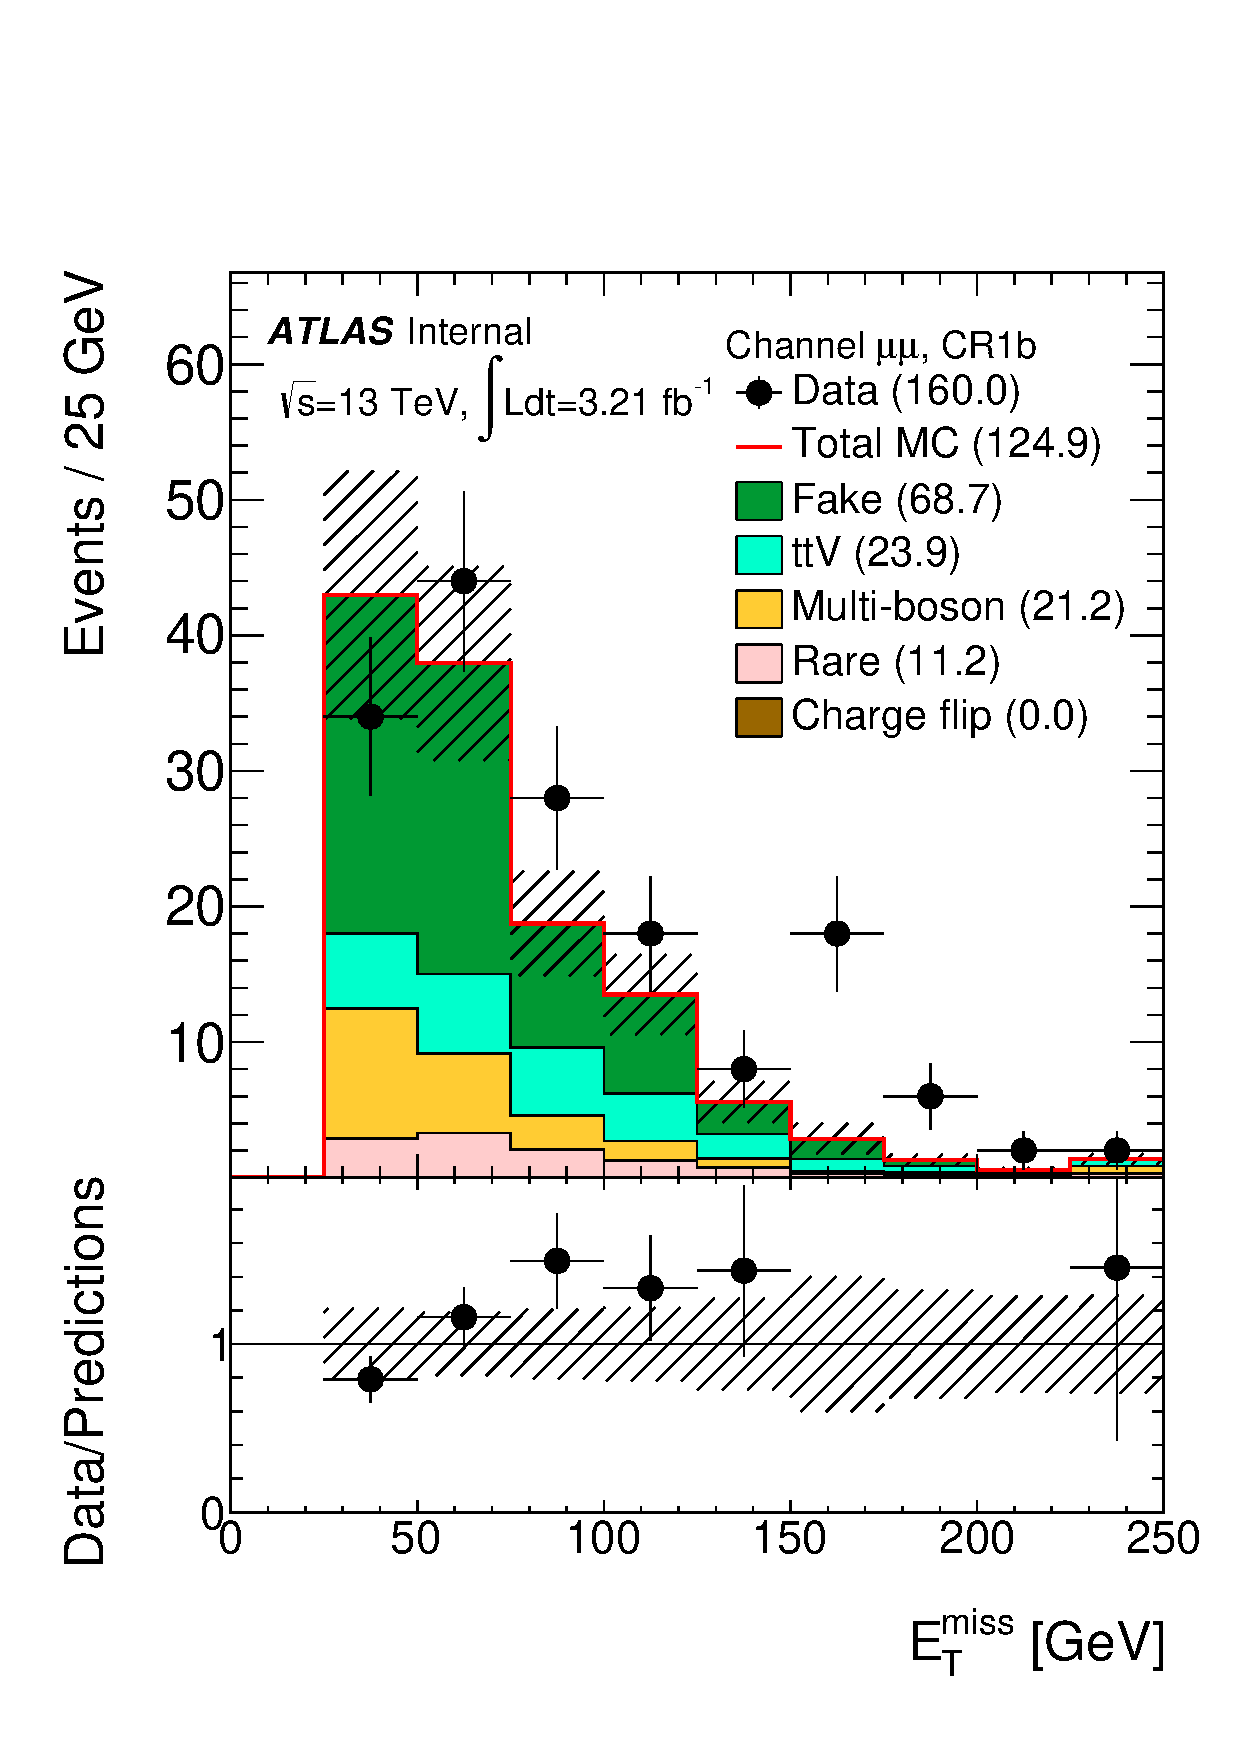
\includegraphics[width=.32\textwidth]{FIGURES/bckg_MC/SS3L/noFit/MET_mm_CR1b_SS3L}
\caption{
Pre-fit distributions for  $ee$ channel (left), for  $e\mu$ channel (middle), and  for  $\mu\mu$ channel (right) from CR1b that were used in the fit to extract the fake rate and charge flip corrections.
 The hashed band represents the sum of systematic uncertainties on the predictions.
\label{f:fit_CR1b}
}
\end{figure}

\begin{figure}[htb]
  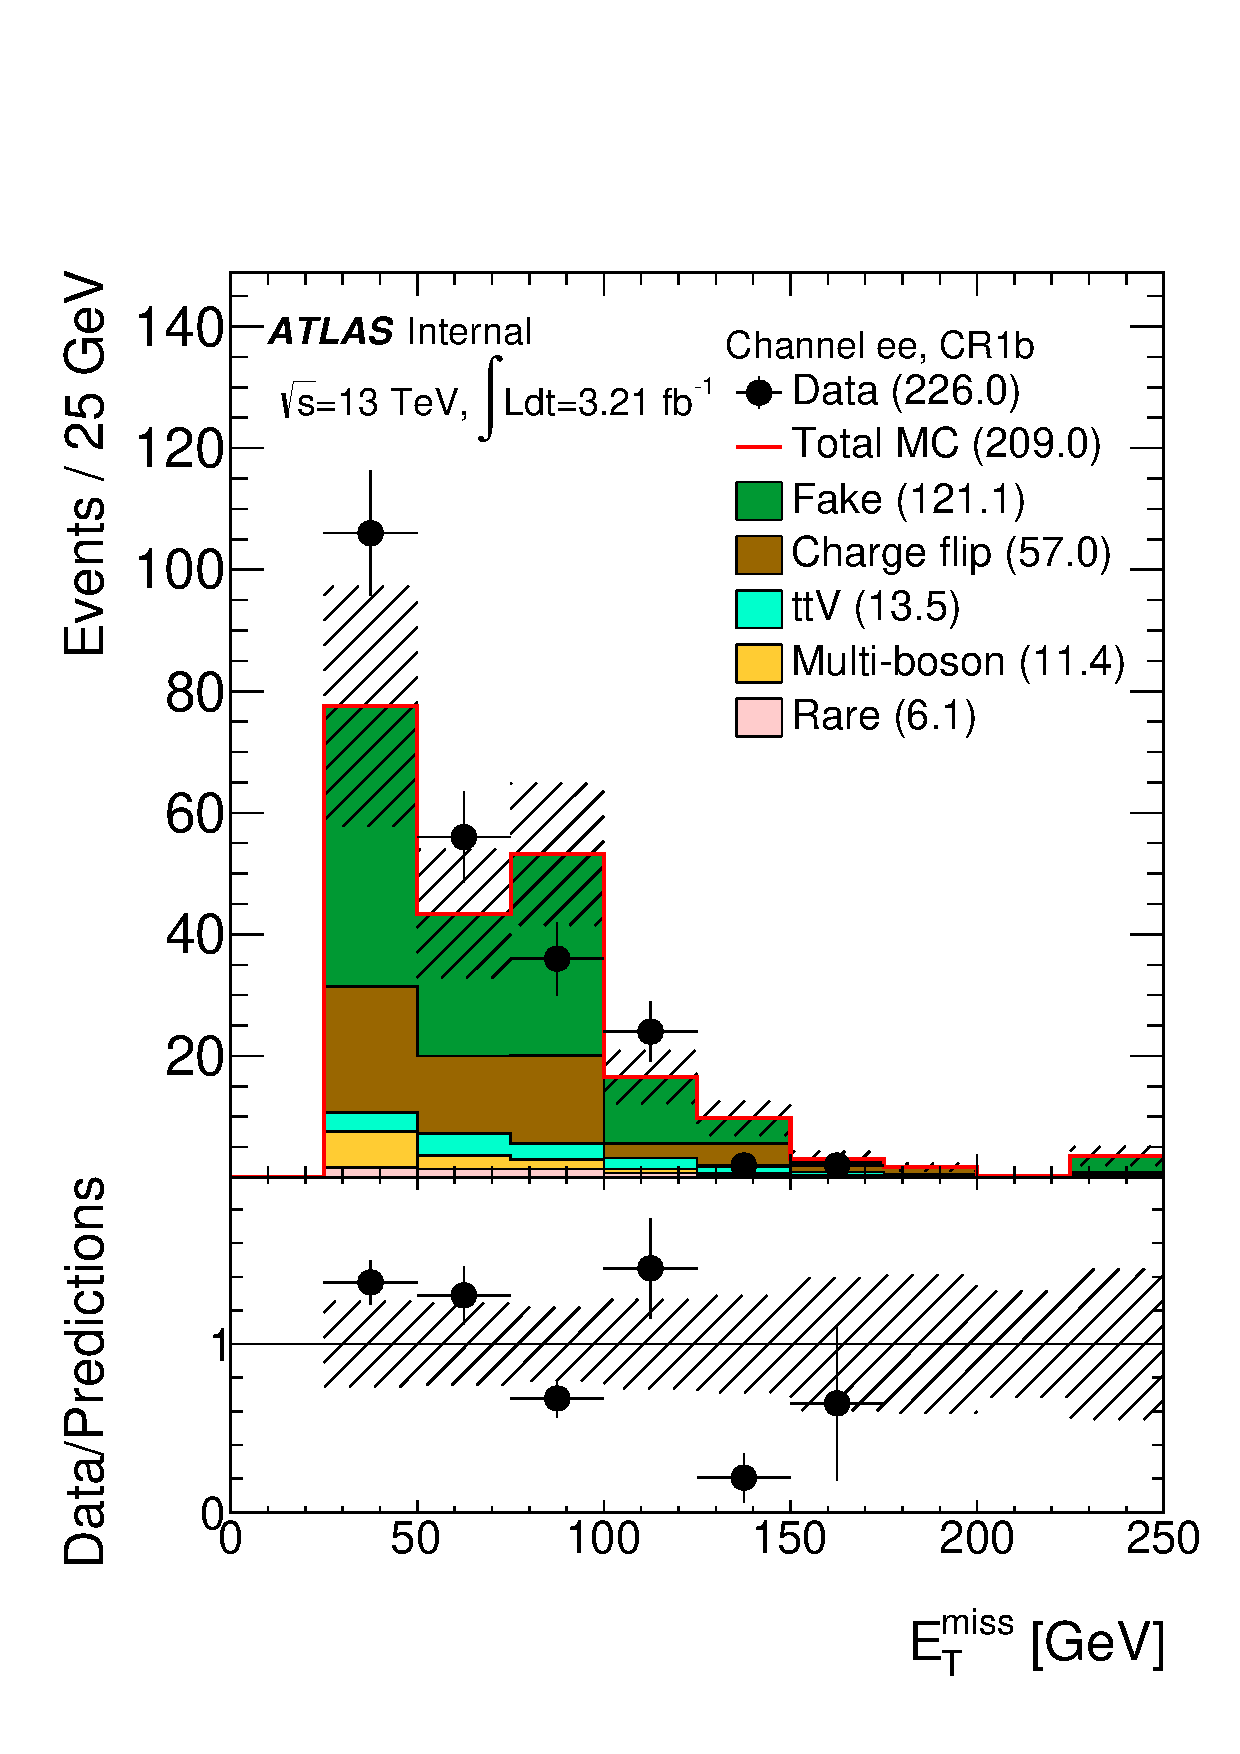
\includegraphics[width=.32\textwidth]{FIGURES/bckg_MC/SS3L/Fit/MET_ee_CR1b_SS3L}
  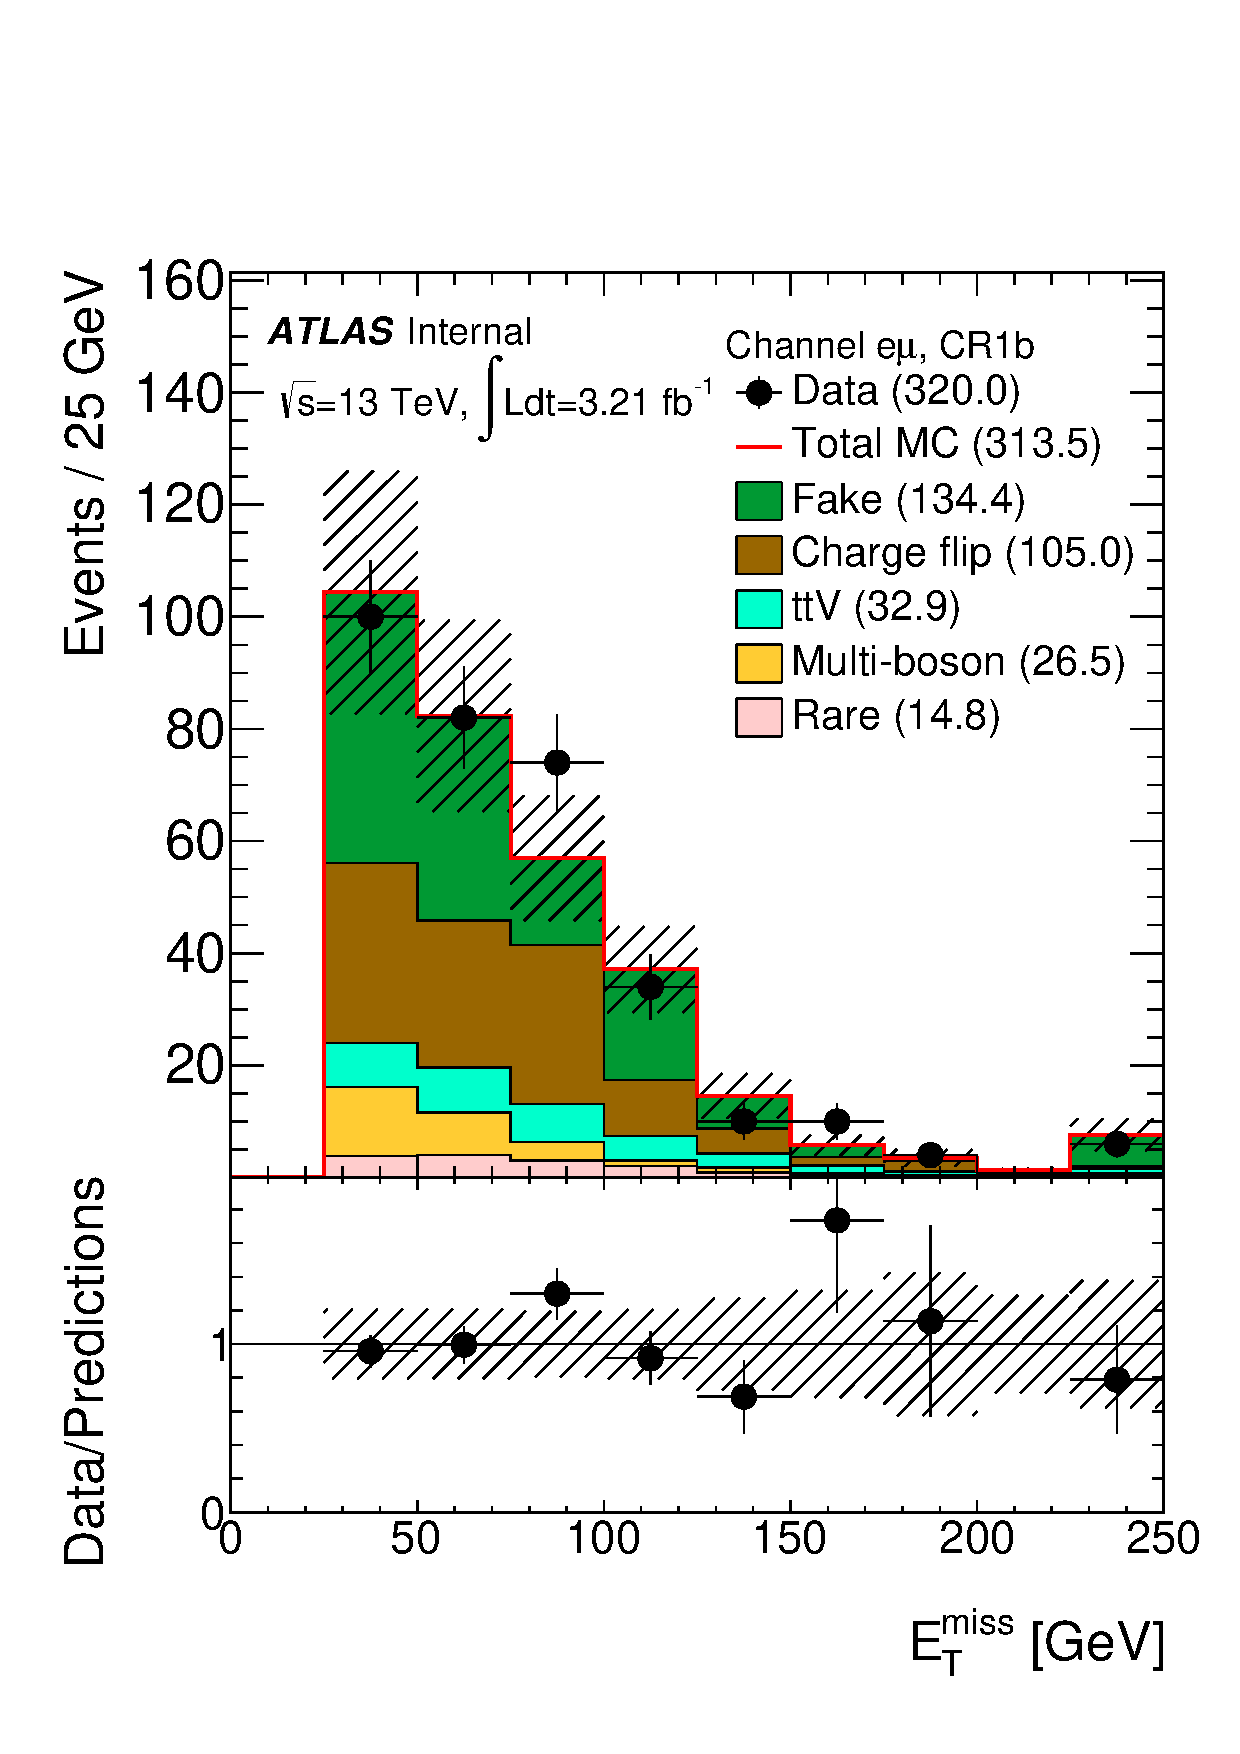
\includegraphics[width=.32\textwidth]{FIGURES/bckg_MC/SS3L/Fit/MET_em_CR1b_SS3L}
  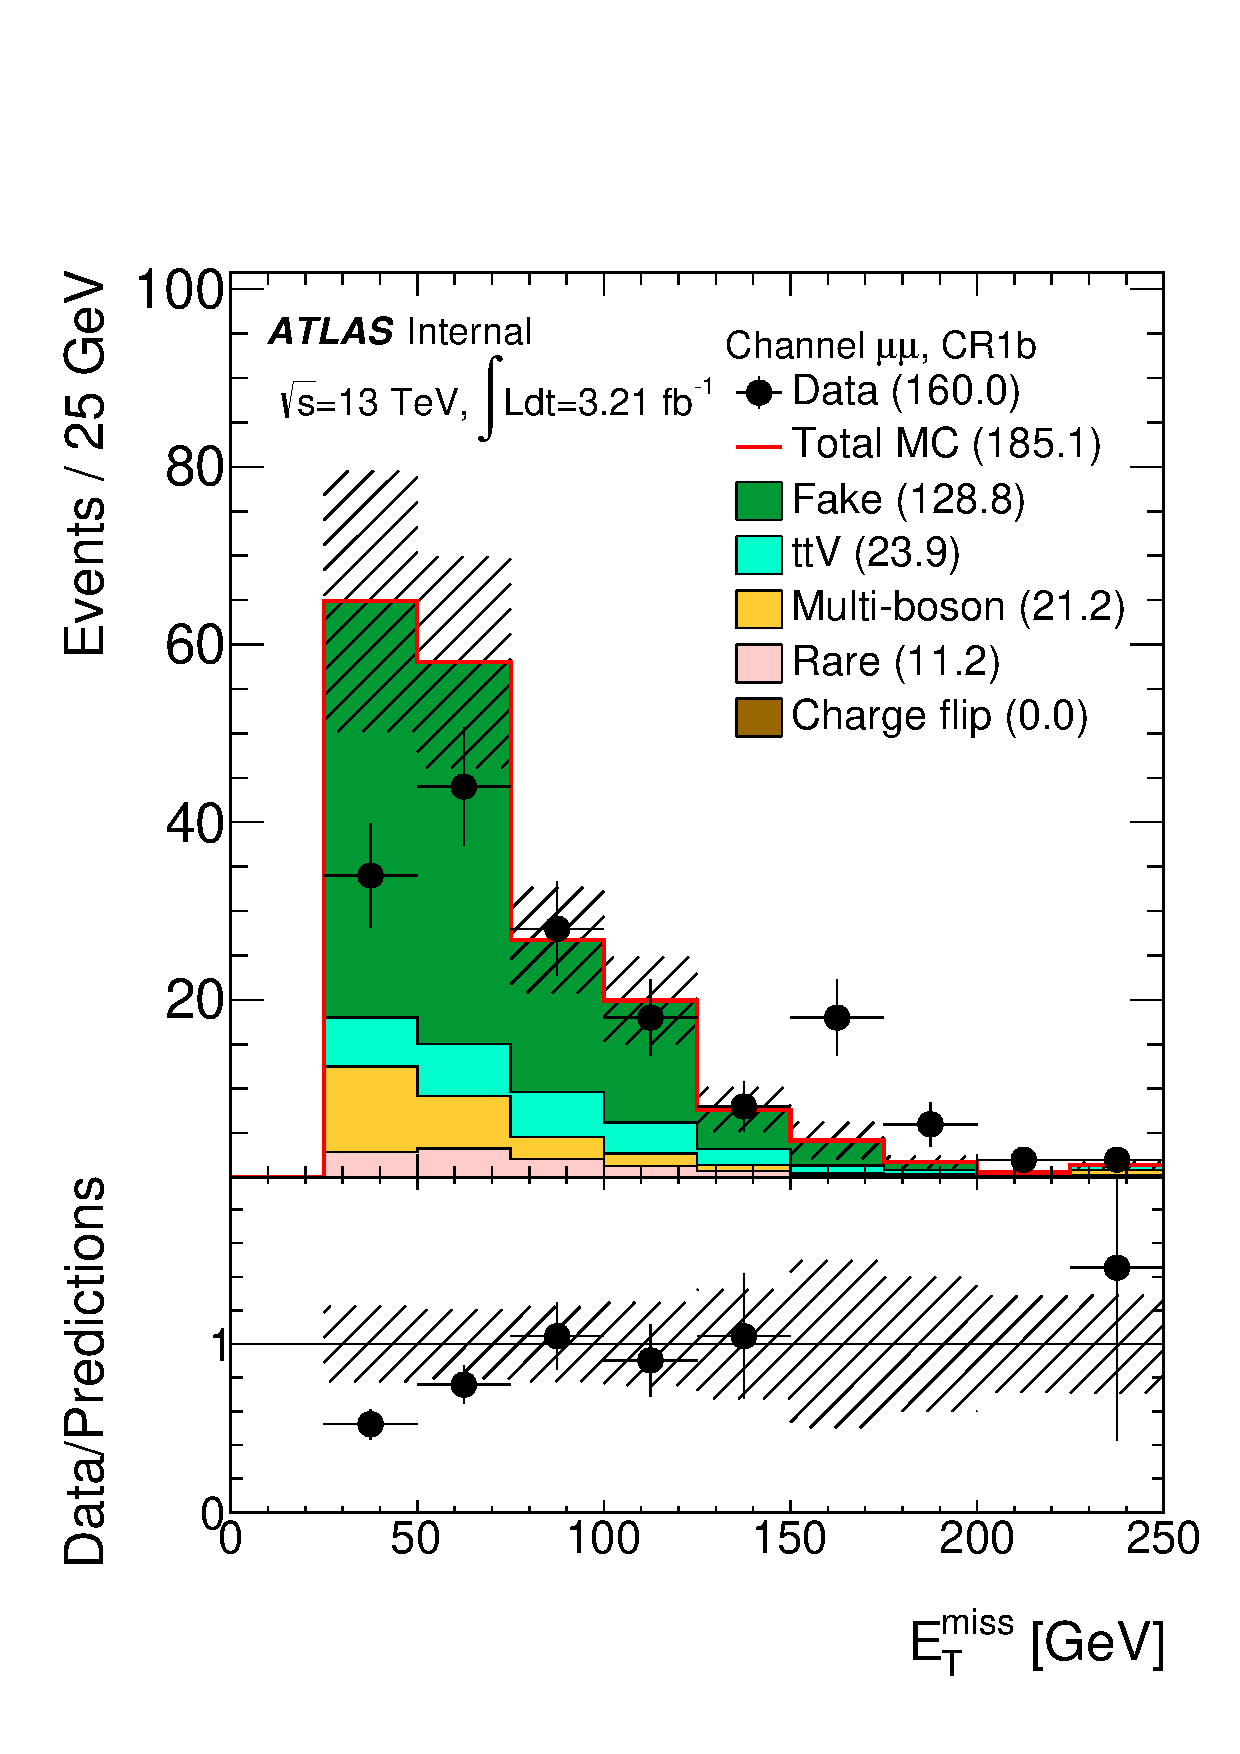
\includegraphics[width=.32\textwidth]{FIGURES/bckg_MC/SS3L/Fit/MET_mm_CR1b_SS3L}
\caption{
Post-fit distributions for  $ee$ channel (left), for  $e\mu$ channel (middle), and  for  $\mu\mu$ channel (right) from CR1b that were used in the fit to extract the fake rate and charge flip corrections.
 The hashed band represents the sum of systematic uncertainties on the predictions.
\label{f:fit_CR1b}
}
\end{figure}

The minimization of the negative log likelihood using the \textsc{Minuit} package leads 
to the correction factors shown in Table \ref{t:fake_factors}. The large uncertainties in the correction factors are due to the limitted amount of data.
The uncertainties in the corrections correspond to how much the parameter needs to be varied for a one standard deviation change in the likelihood function. 
This uncertainty takes into account the limited number of simulated events and is included as a systematic uncertainty on the expected number of background events. 

\begin{table}[htb]
  \caption{The fake-rate and charge flip corrections obtained after minimizing the likelihood function.
The uncertainty in the corrections takes into account the limited statistics of simulated events.
  \label{t:fake_factors}}
  \centering
%  \scalebox{0.85}{                                                                                                                                                                                                                    
  \begin{tabular}{|c|c|c|}
    \hline
    Category & Correction & Uncertainty  \\
    \hline
    Charge Flip        &    1.04    &   0.21    \\
    EL HF              &    2.26    &   0.68    \\
    EL LF              &    1.06    &   0.21    \\
    MU HF              &    1.88    &   0.22    \\
    MU LF              &    0.00    &   0.18    \\
    \hline
  \end{tabular}
 % }                                                                            
 \end{table}

Distributions other than the six shown in Figures \ref{f:fit_CR0b}-\ref{f:fit_CR1b} were used to validate the accuracy of the simulations 
and are shown in Figures \ref{f:val_met_CR0b}-\ref{f:val_met_CR1b}. 
The electron-electron channel in both control regions provides a good handle on the charge flip background due to the large number of events classified as charge flip.  
The fake electrons from heavy-flavor jets are constrained in the CR1b, while the fake electrons contributions from light-flavor jets are eliminated after the fit due to the lack of events in this category. 
Data and predictions in the control regions after correcting the rates of non-prompt leptons and charge flip agree within uncertainties.

\begin{figure}[htb]
 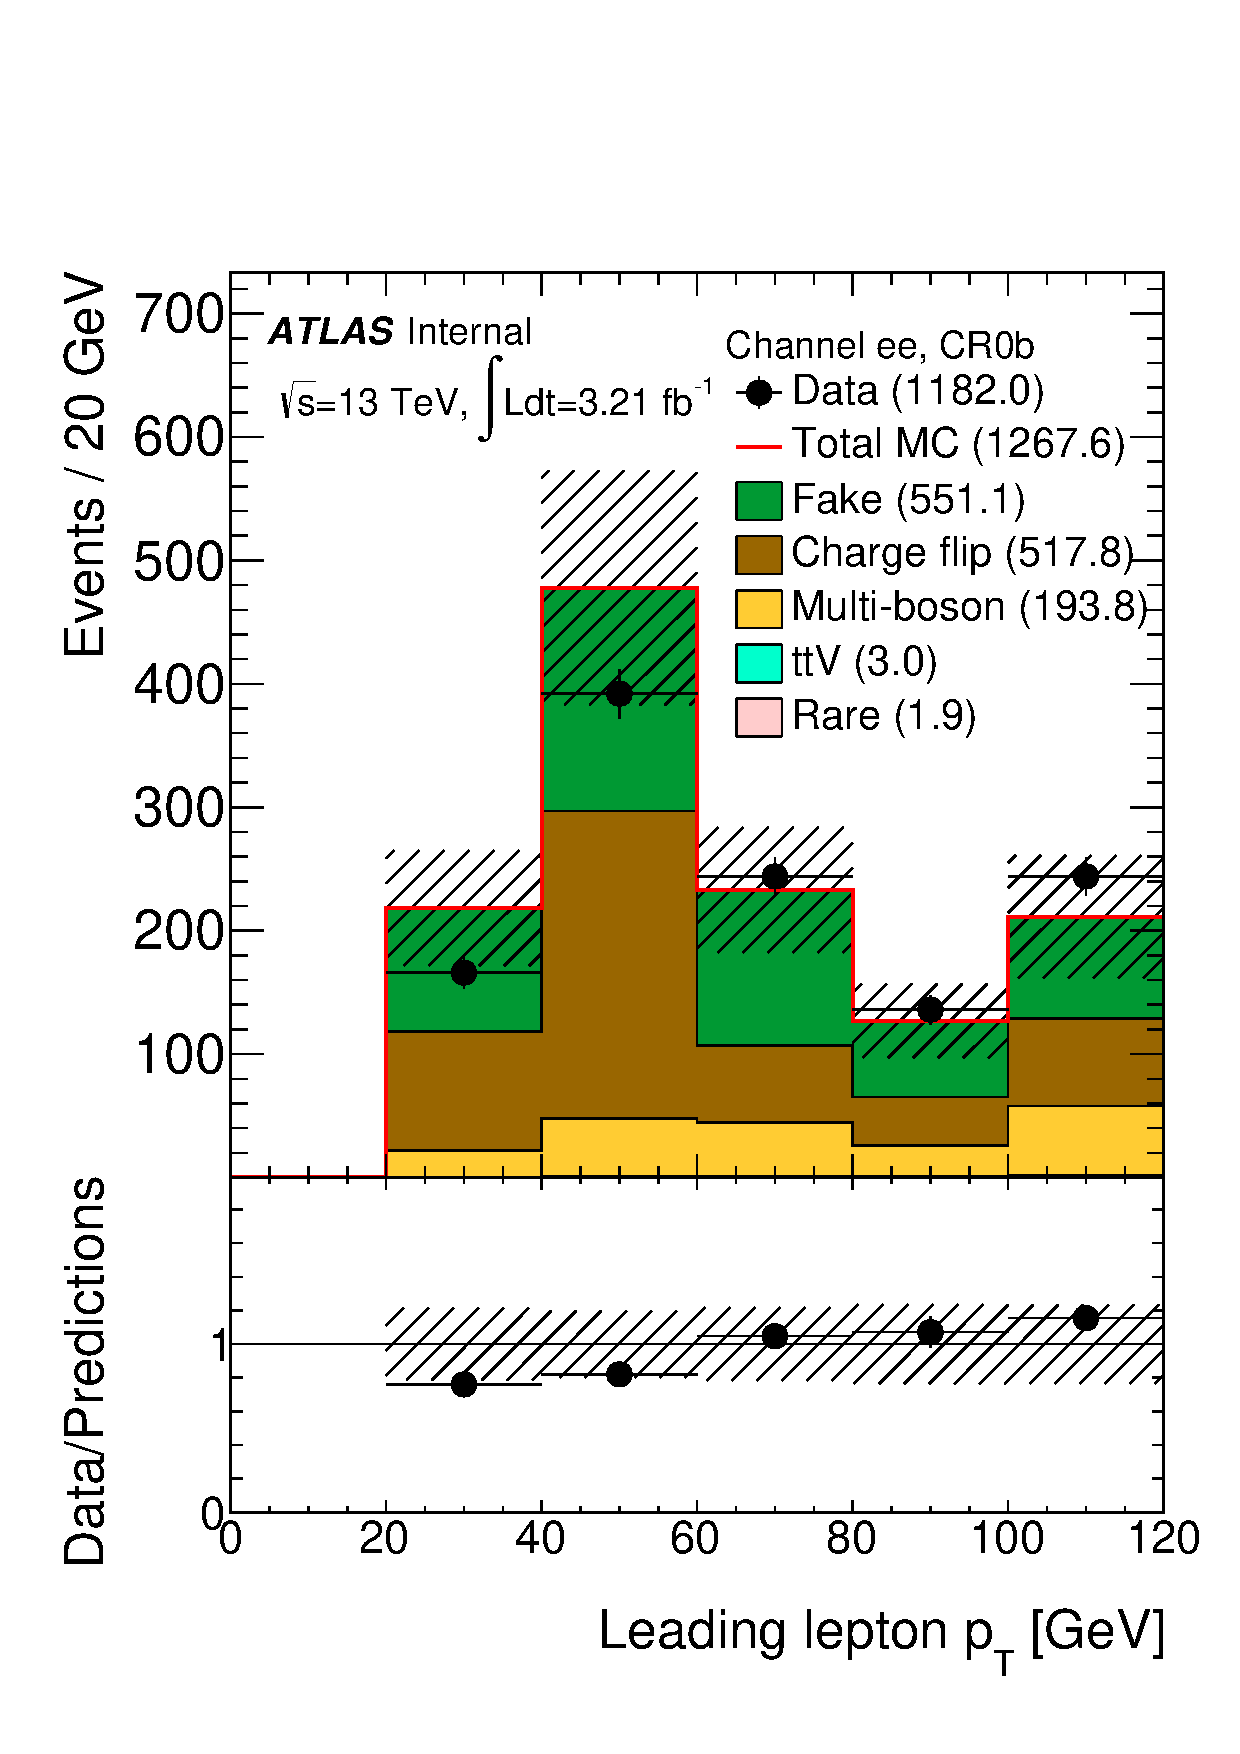
\includegraphics[width=.32\textwidth]{FIGURES/bckg_MC/SS3L/Fit/LEP1Pt_ee_CR0b_SS3L}
  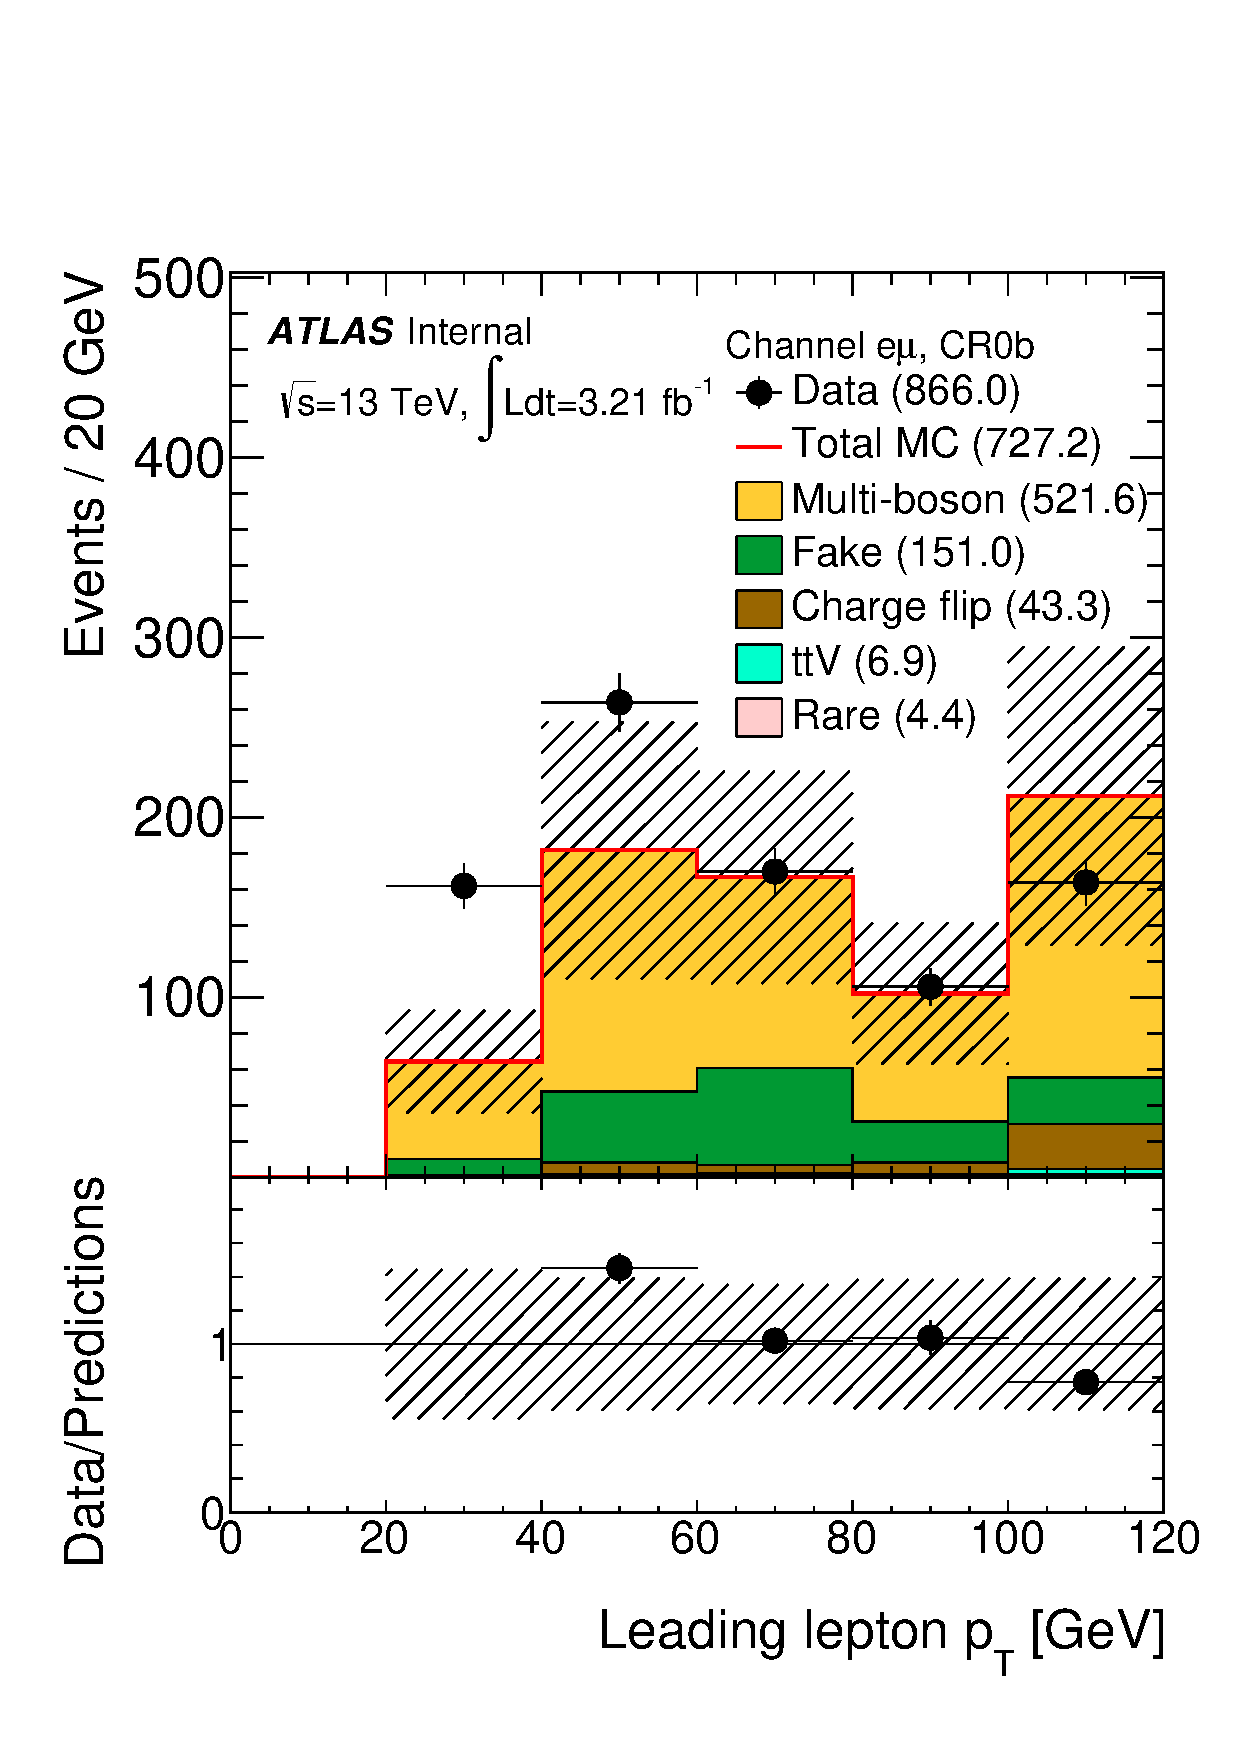
\includegraphics[width=.32\textwidth]{FIGURES/bckg_MC/SS3L/Fit/LEP1Pt_em_CR0b_SS3L}
  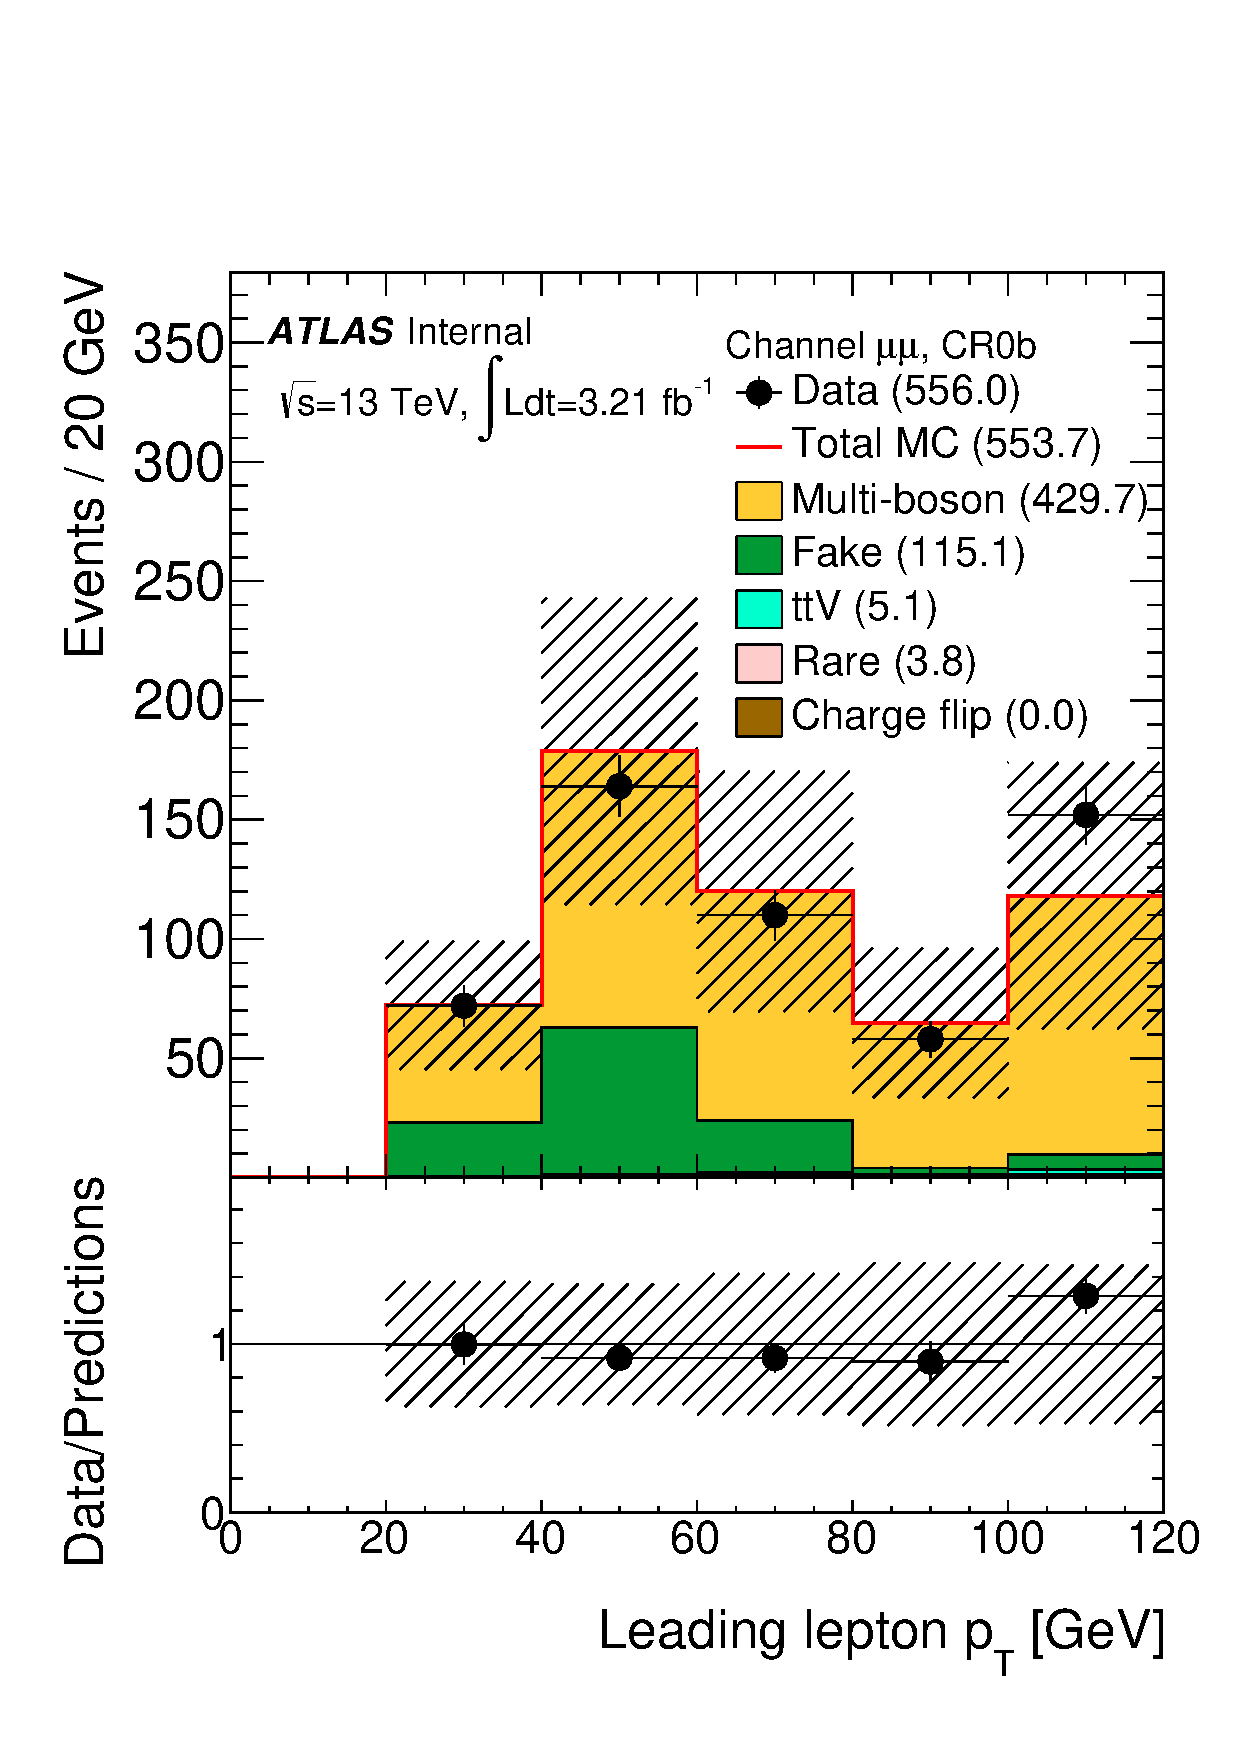
\includegraphics[width=.32\textwidth]{FIGURES/bckg_MC/SS3L/Fit/LEP1Pt_mm_CR0b_SS3L}
\caption{
Post-fit distributions of the leading lepton $p_T$ for CR0b for $ee$ channel (left), $e\mu$ channel (middle), and $\mu\mu$ channel (right)  used to validate the accuracy of the simulation.
Fake-rate and charge flip corrections are applied to these distributions. The hashed band represents the sum of systematic uncertainties on the predictions.
\label{f:val_met_CR0b}
}
\end{figure}

\begin{figure}[htb]
 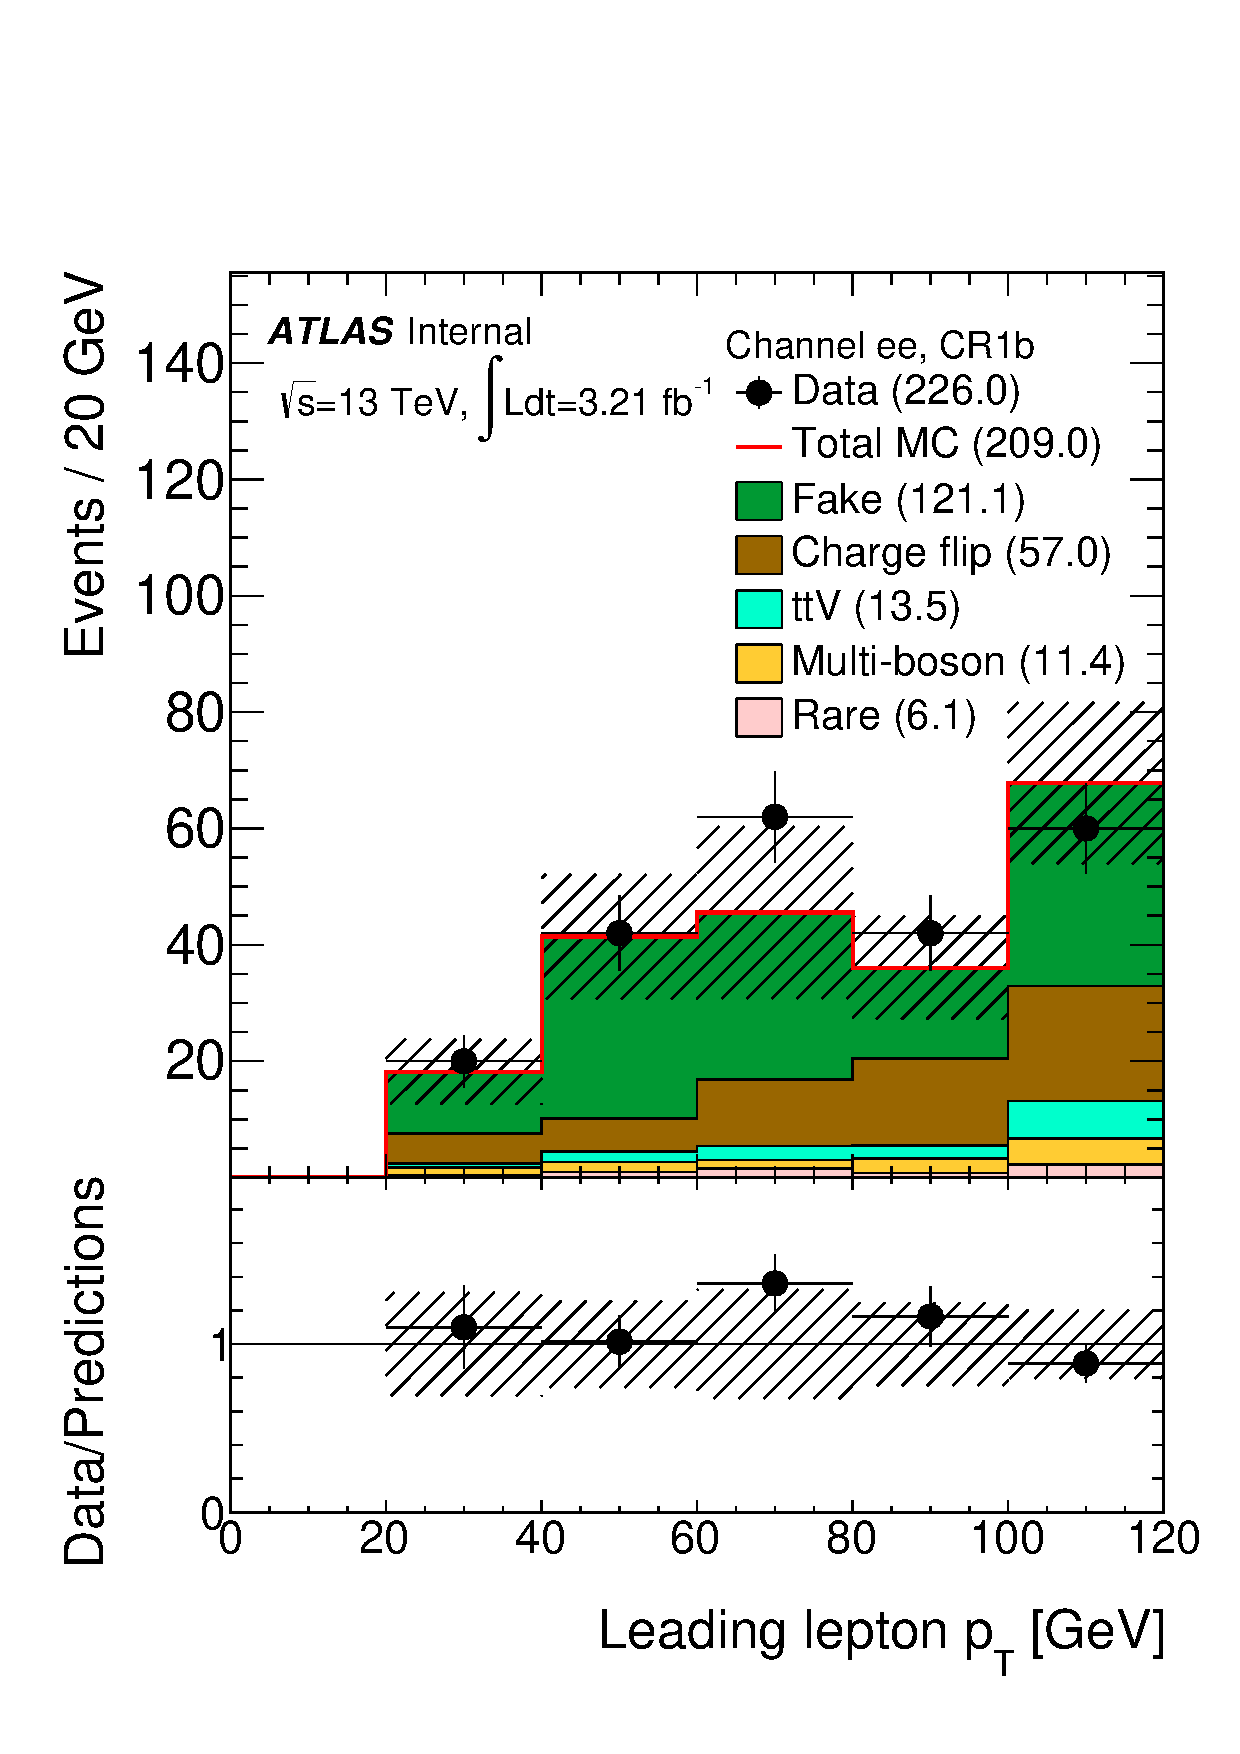
\includegraphics[width=.32\textwidth]{FIGURES/bckg_MC/SS3L/Fit/LEP1Pt_ee_CR1b_SS3L}
  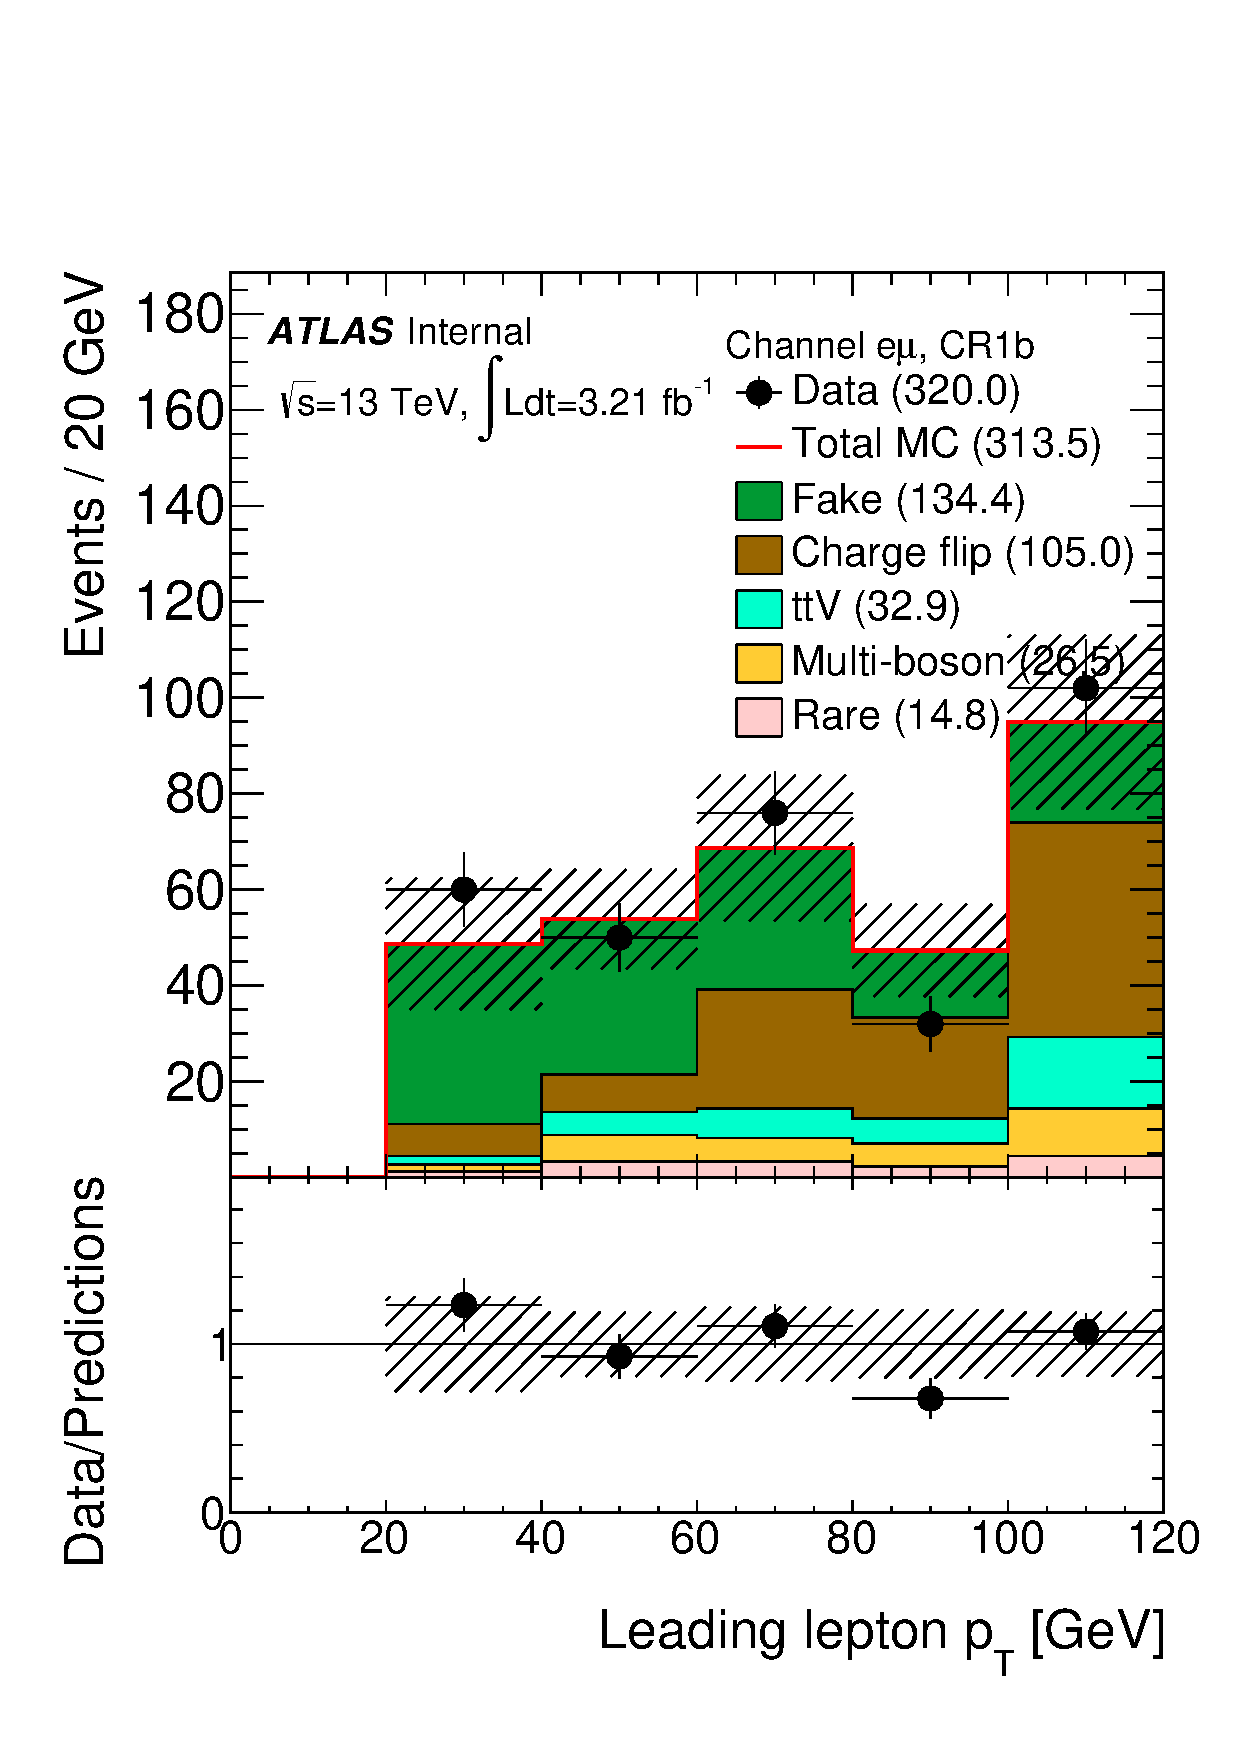
\includegraphics[width=.32\textwidth]{FIGURES/bckg_MC/SS3L/Fit/LEP1Pt_em_CR1b_SS3L}
  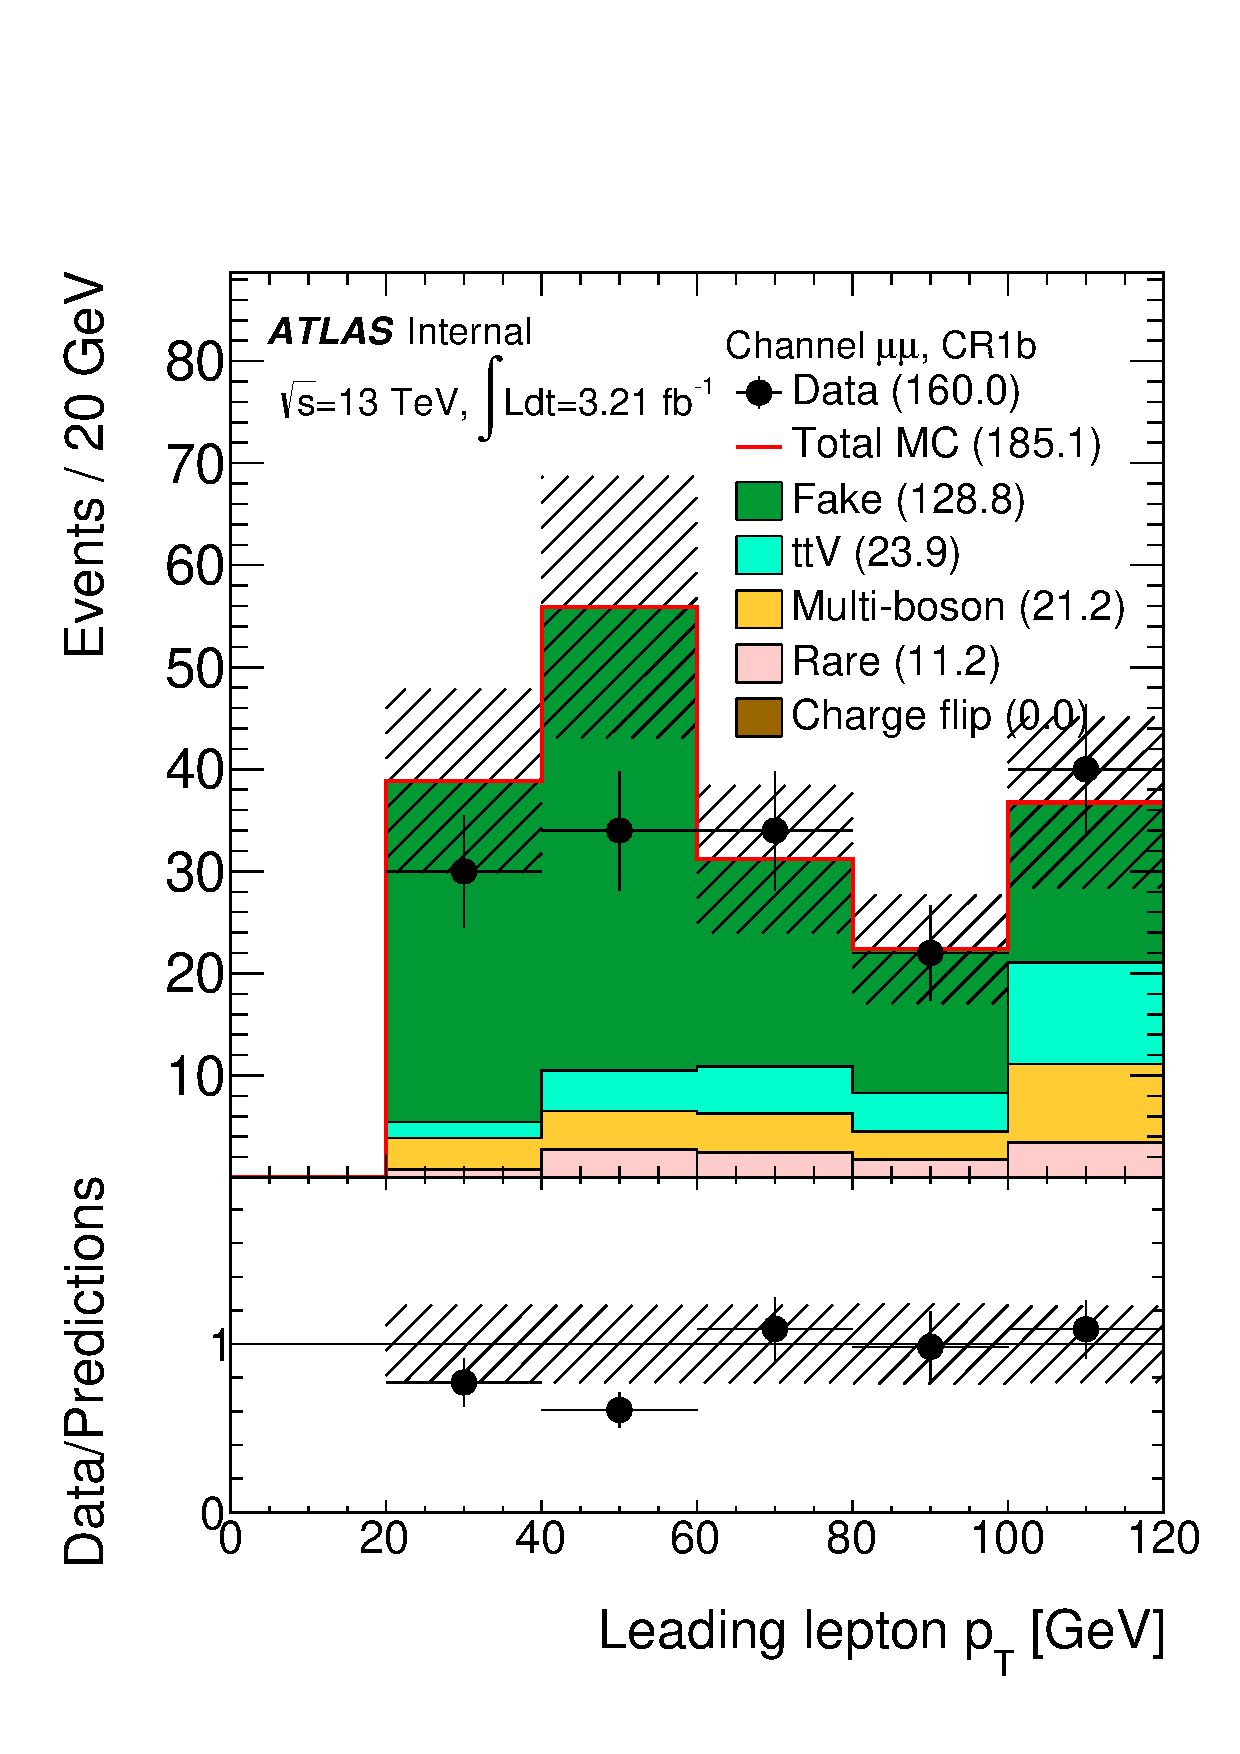
\includegraphics[width=.32\textwidth]{FIGURES/bckg_MC/SS3L/Fit/LEP1Pt_mm_CR1b_SS3L}
\caption{
Post-fit distributions of the leading lepton $p_T$ for CR1b for $ee$ channel (left), $e\mu$ channel (middle), and $\mu\mu$ channel (right)  used to validate the accuracy of the simulation.
Fake-rate and charge flip corrections are applied to these distributions. The hashed band represents the sum of systematic uncertainties on the predictions.
\label{f:val_met_CR1b}
}
\end{figure}


\begin{figure}[htb]
\centering
 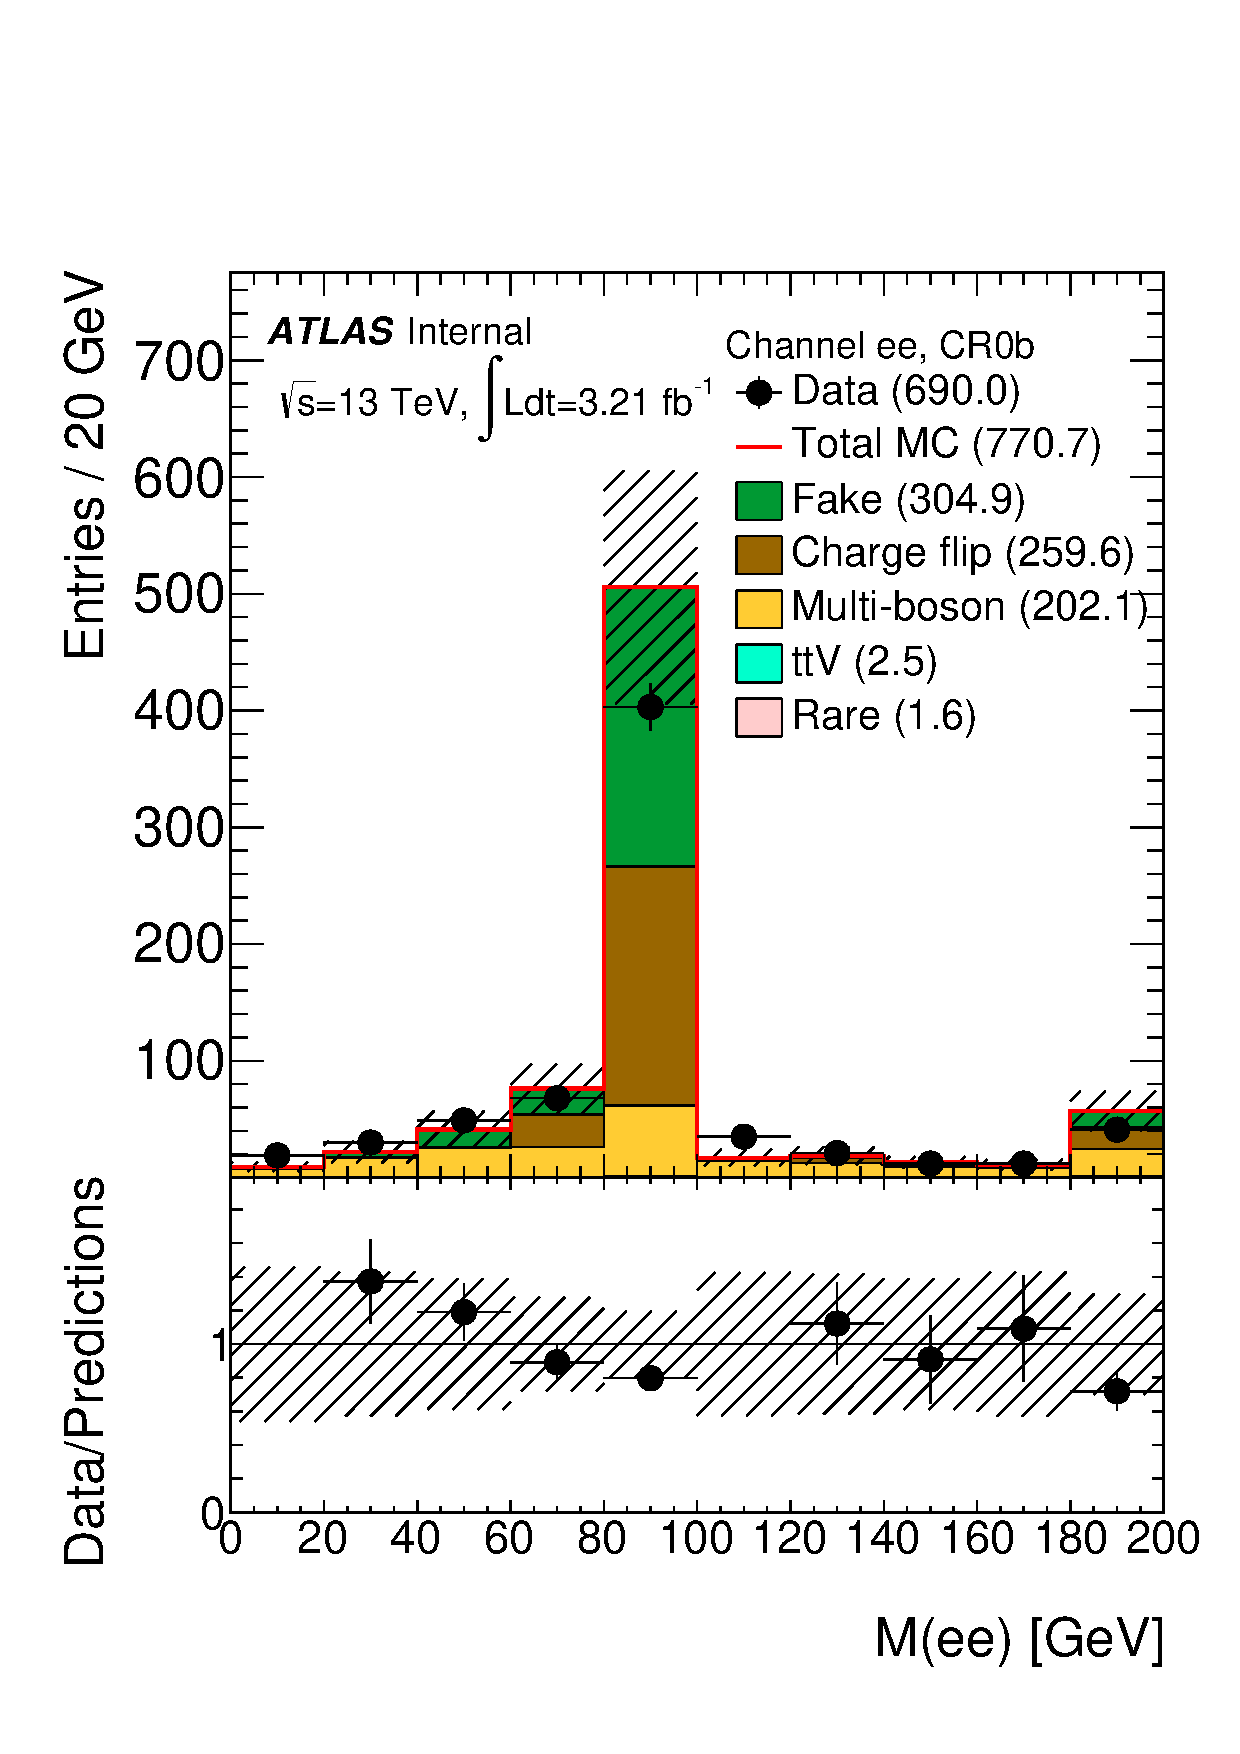
\includegraphics[width=.32\textwidth]{FIGURES/bckg_MC/SS3L/Fit/Mee_ee_CR0b_SS3L}
  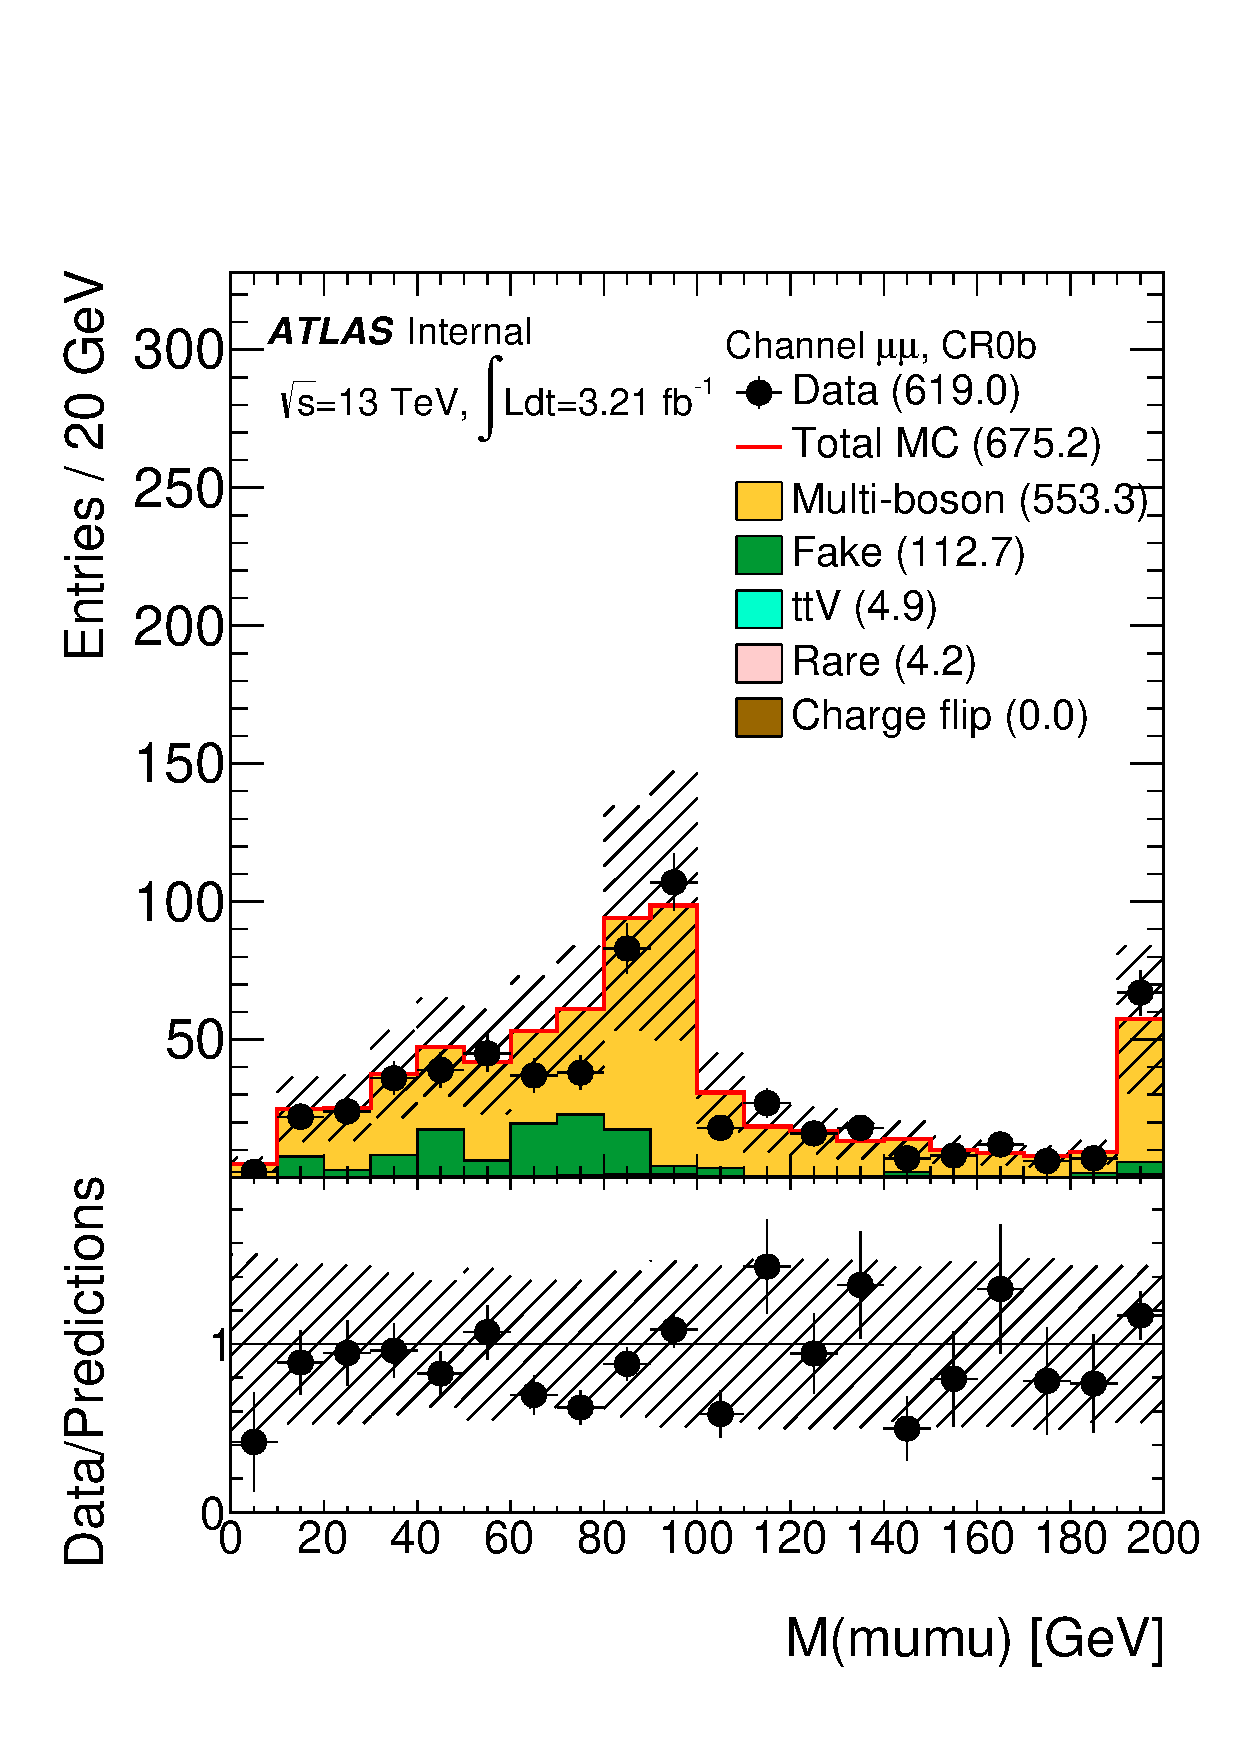
\includegraphics[width=.32\textwidth]{FIGURES/bckg_MC/SS3L/Fit/Mmumu_mm_CR0b_SS3L}
\caption{
Post-fit distributions of the invariant mass of two leptons for CR0b for $ee$ channel (left) and $\mu\mu$ channel (right)  used to validate the accuracy of the simulation.
Fake-rate and charge flip corrections are applied to these distributions. The hashed band represents the sum of systematic uncertainties on the predictions.
\label{f:val_met_CR0b}
}
\end{figure}



\begin{figure}[htb]
\centering
 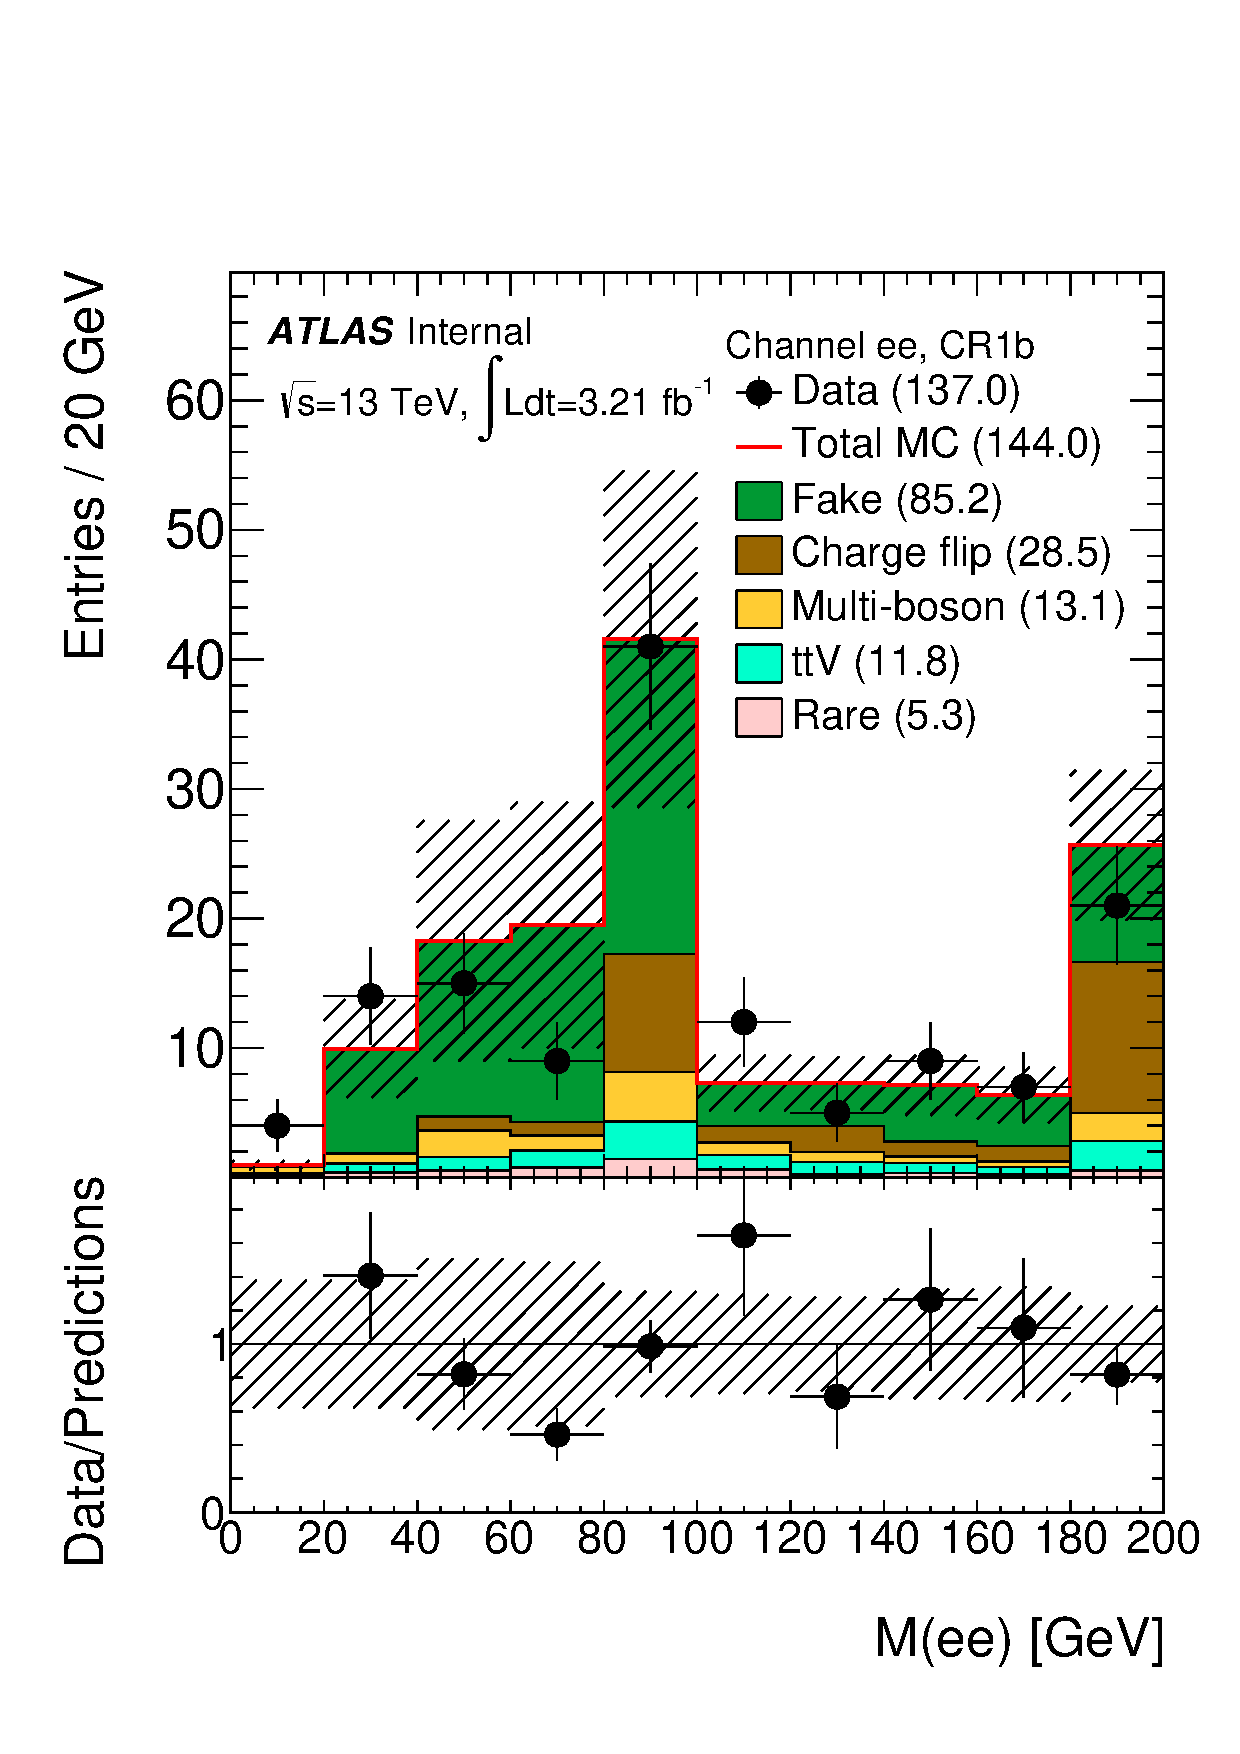
\includegraphics[width=.32\textwidth]{FIGURES/bckg_MC/SS3L/Fit/Mee_ee_CR1b_SS3L}
  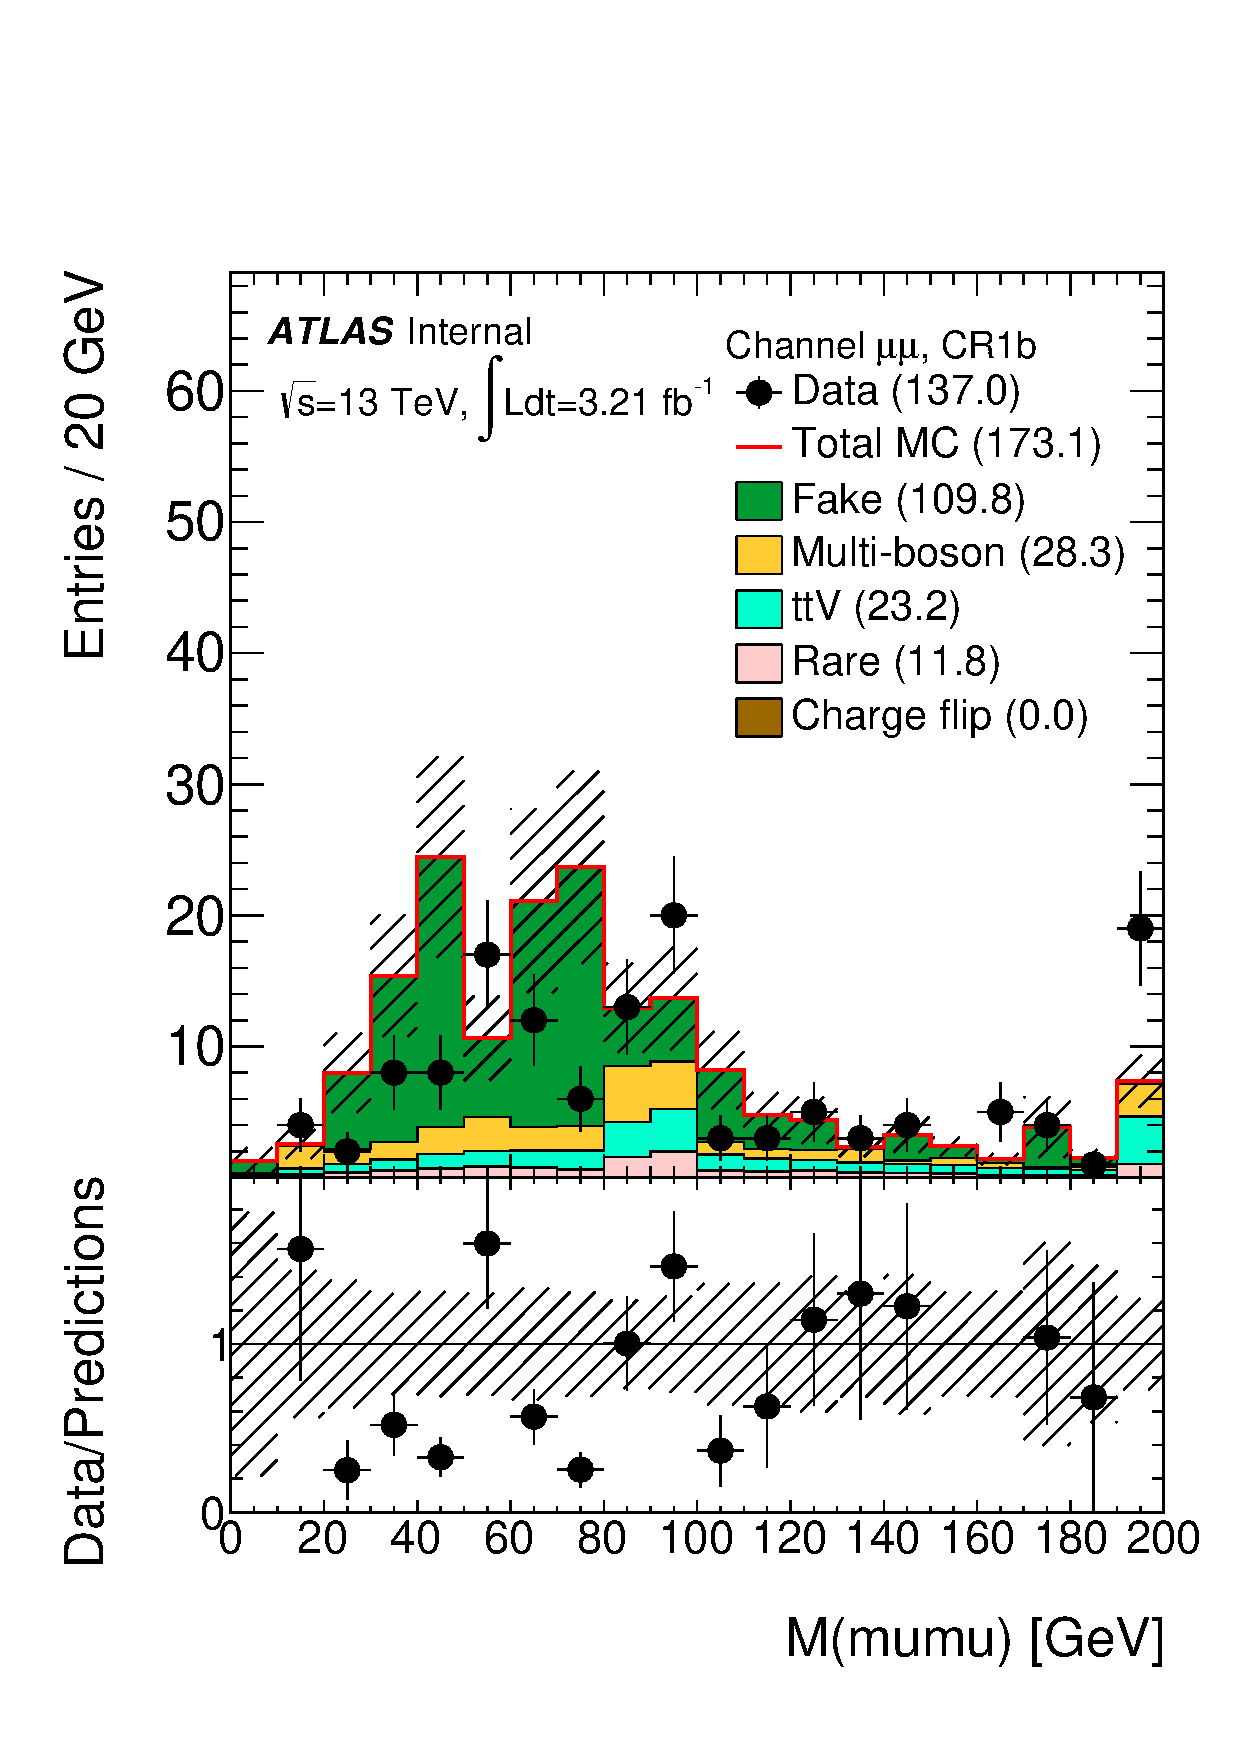
\includegraphics[width=.32\textwidth]{FIGURES/bckg_MC/SS3L/Fit/Mmumu_mm_CR1b_SS3L}
\caption{
Post-fit distributions of the invariant mass of two leptons for CR1b for $ee$ channel (left) and $\mu\mu$ channel (right)  used to validate the accuracy of the simulation.
Fake-rate and charge flip corrections are applied to these distributions. The hashed band represents the sum of systematic uncertainties on the predictions.
\label{f:val_met_CR1b}
}
\end{figure}


\begin{figure}[htb]
 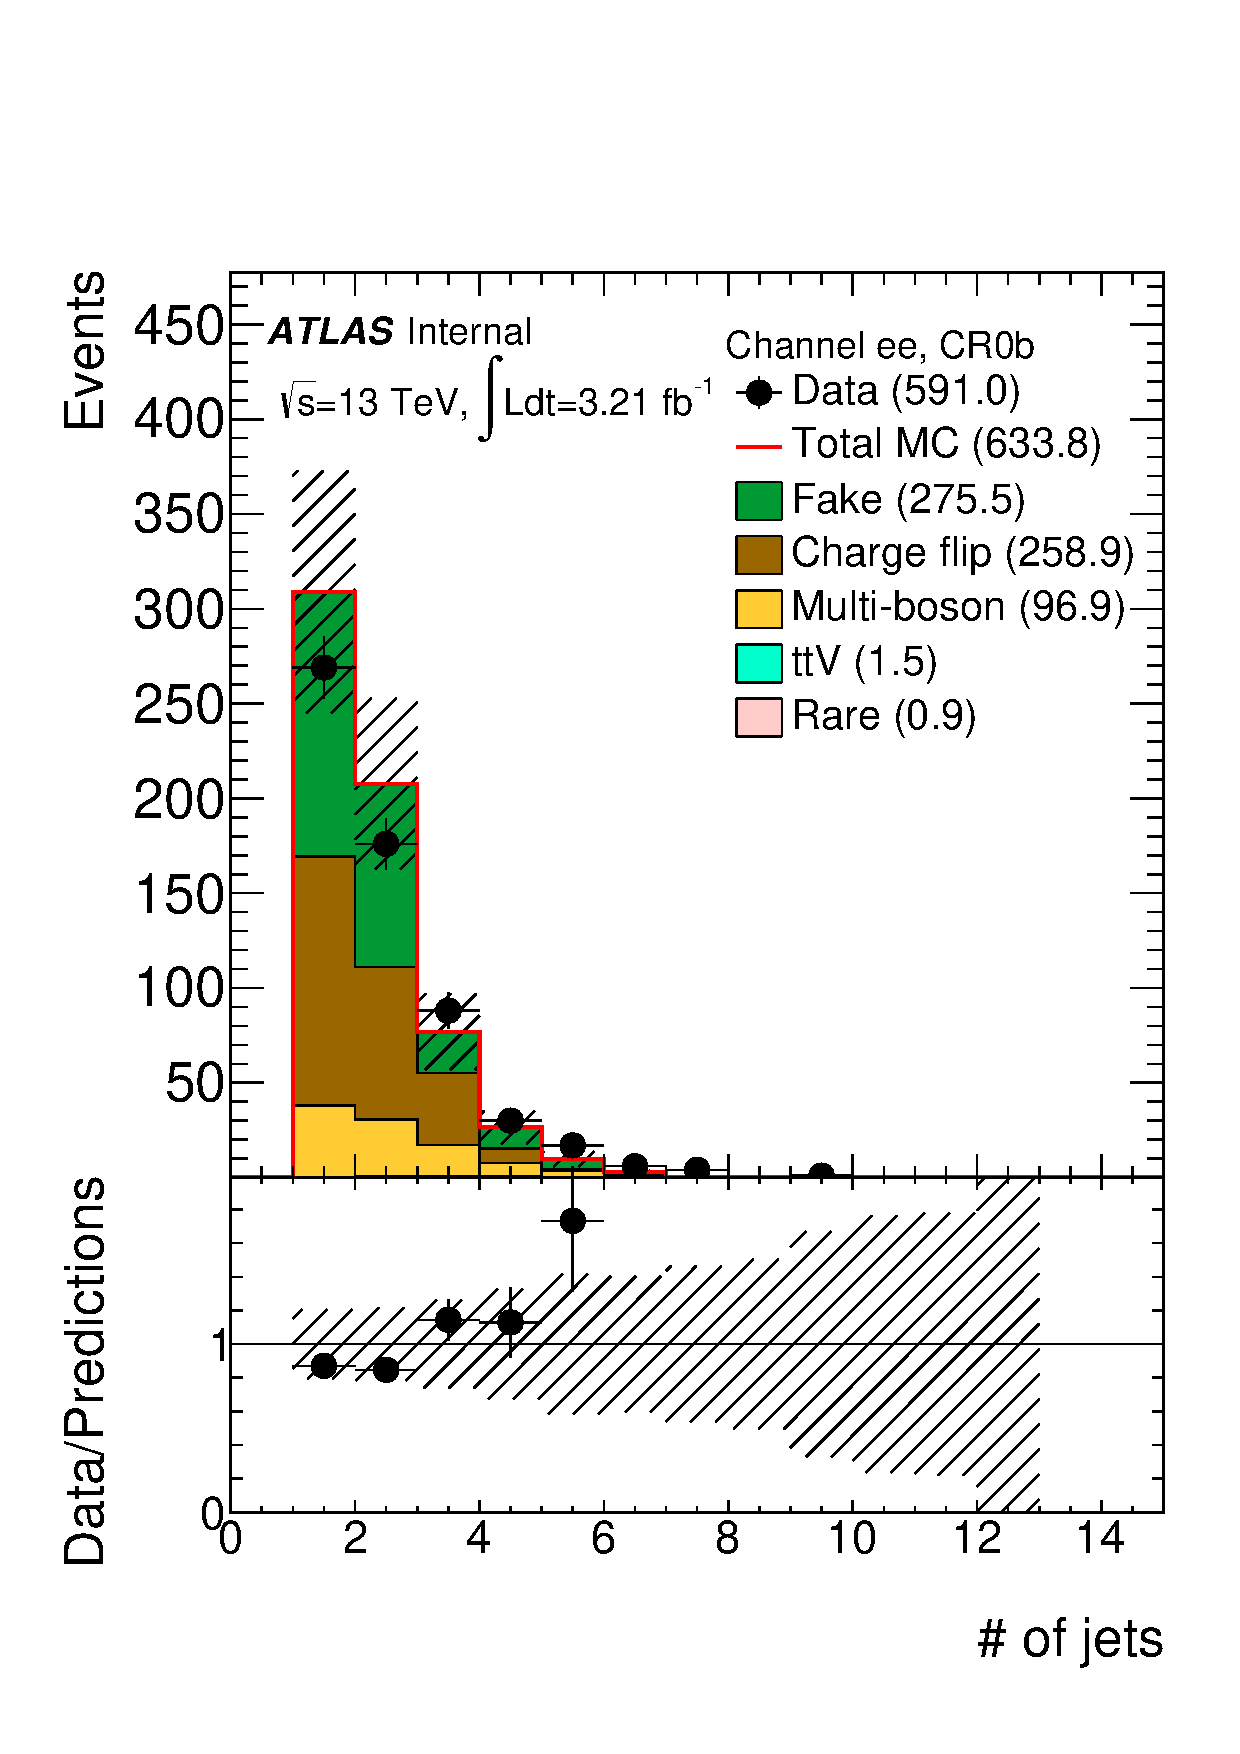
\includegraphics[width=.32\textwidth]{FIGURES/bckg_MC/SS3L/Fit/NJETS_ee_CR0b_SS3L}
  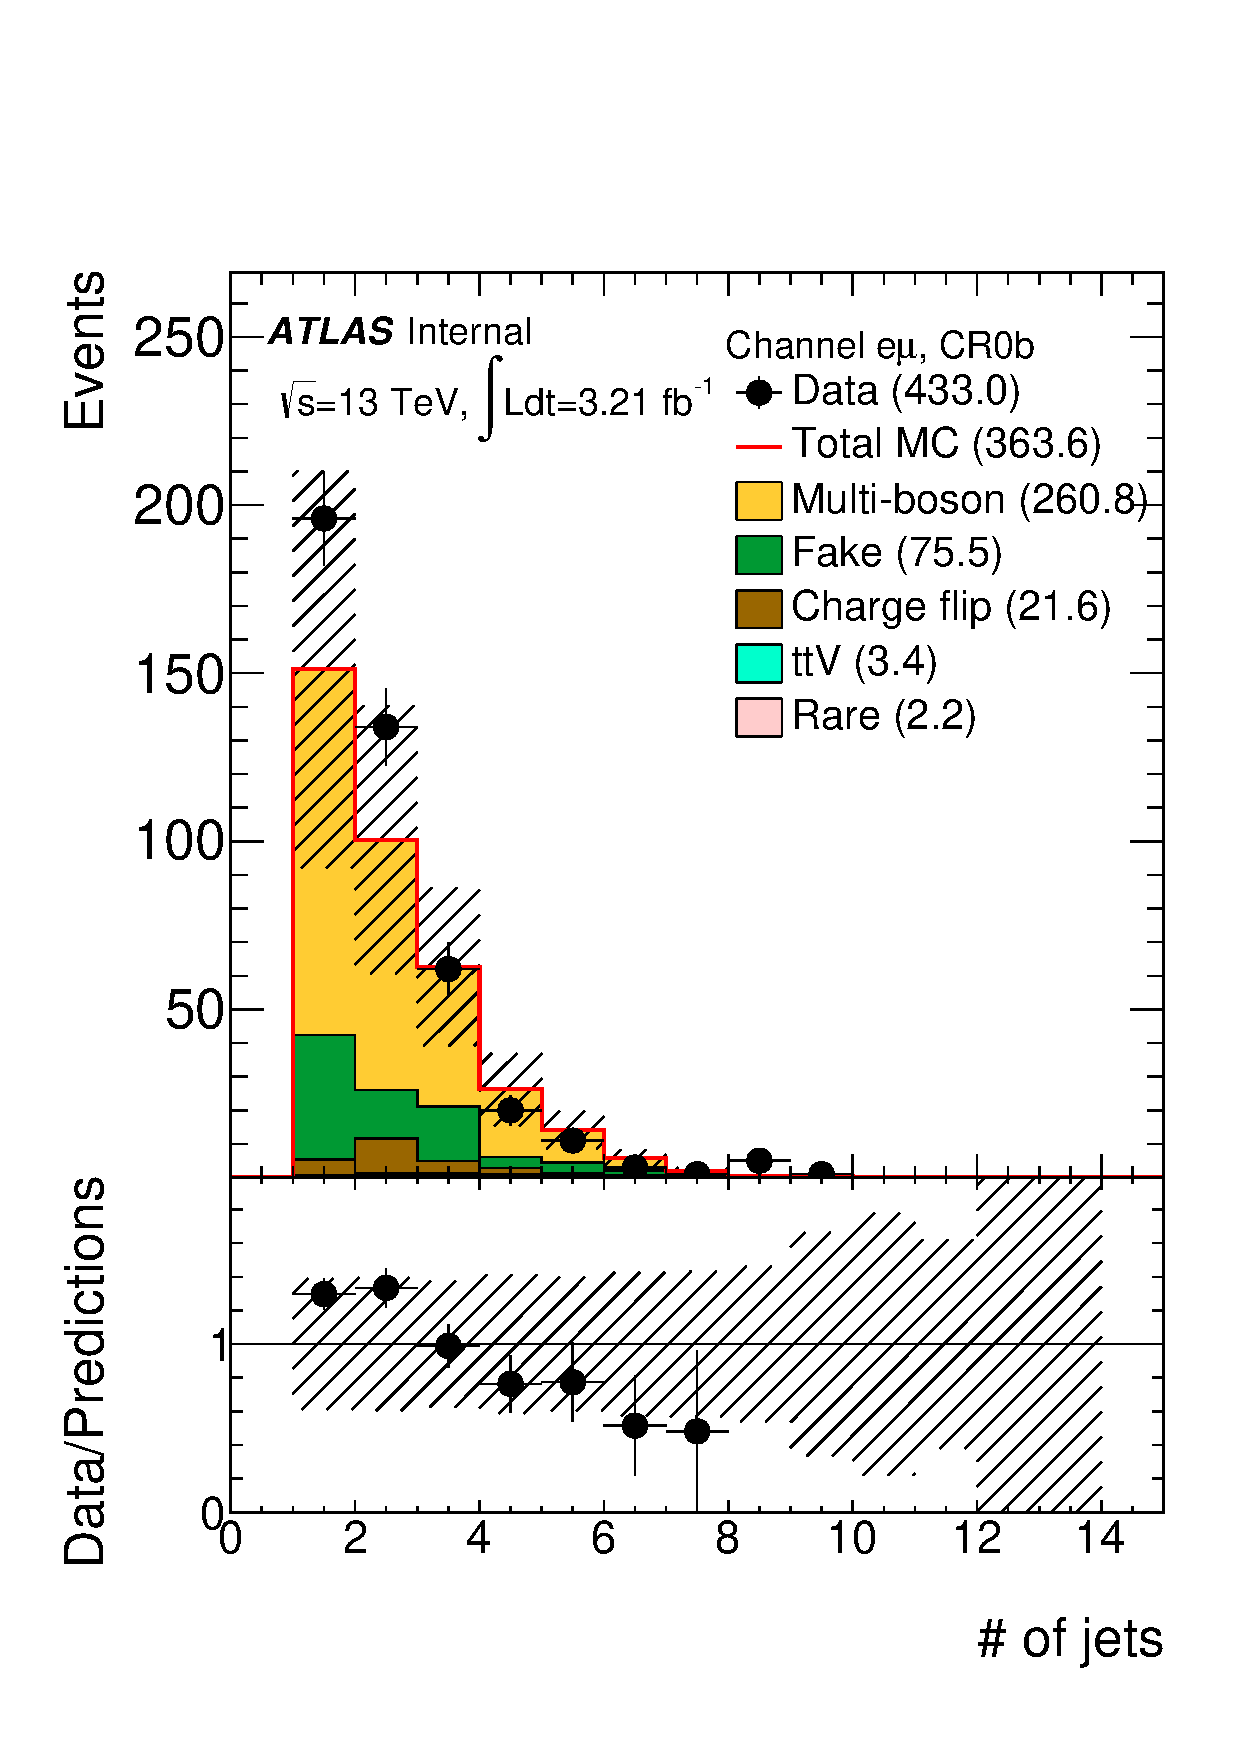
\includegraphics[width=.32\textwidth]{FIGURES/bckg_MC/SS3L/Fit/NJETS_em_CR0b_SS3L}
  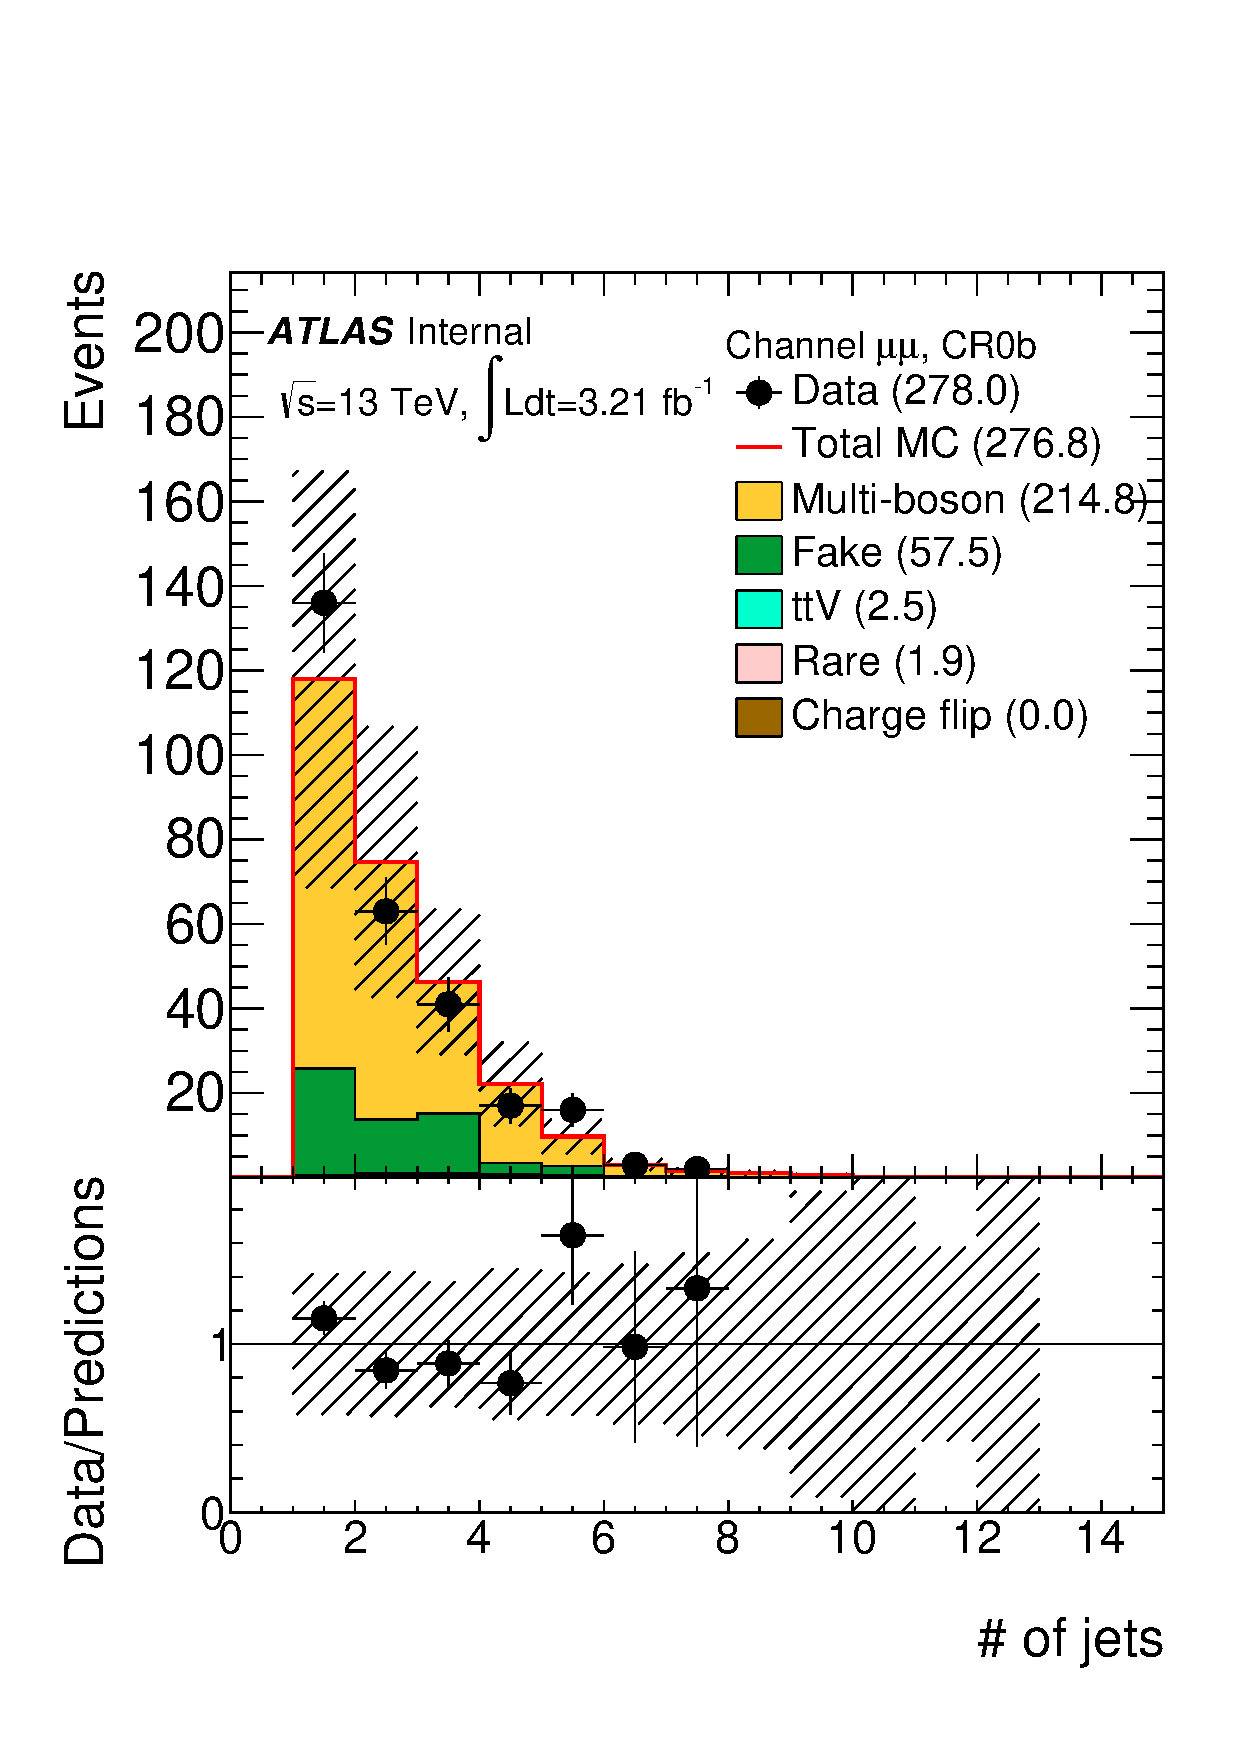
\includegraphics[width=.32\textwidth]{FIGURES/bckg_MC/SS3L/Fit/NJETS_mm_CR0b_SS3L}
\caption{
Post-fit distributions of the transverse mass for CR0b for $ee$ channel (left), $e\mu$ channel (middle), and $\mu\mu$ channel (right)  used to validate the accuracy of the simulation.
Fake-rate and charge flip corrections are applied to these distributions. The hashed band represents the sum of systematic uncertainties on the predictions.
\label{f:val_met_CR0b}
}
\end{figure}

\begin{figure}[htb]
 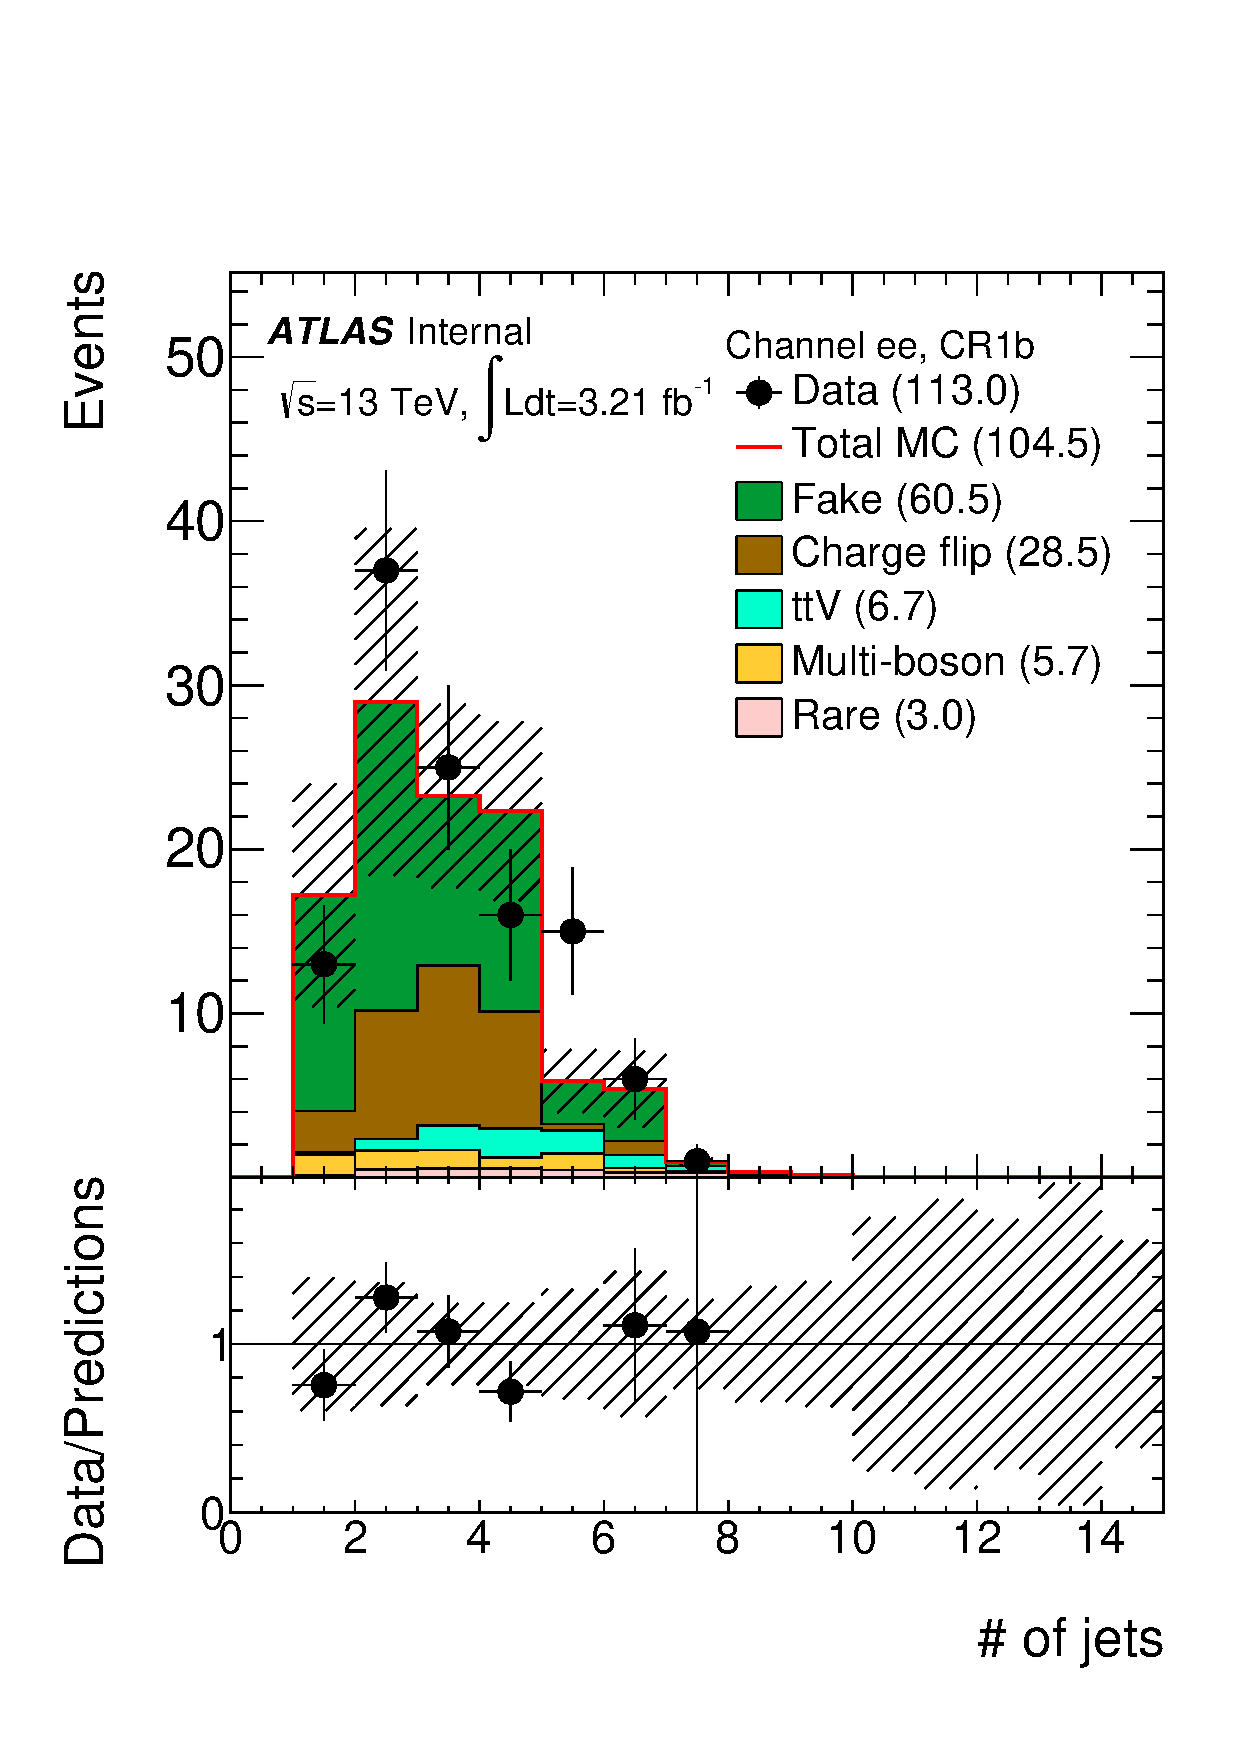
\includegraphics[width=.32\textwidth]{FIGURES/bckg_MC/SS3L/Fit/NJETS_ee_CR1b_SS3L}
  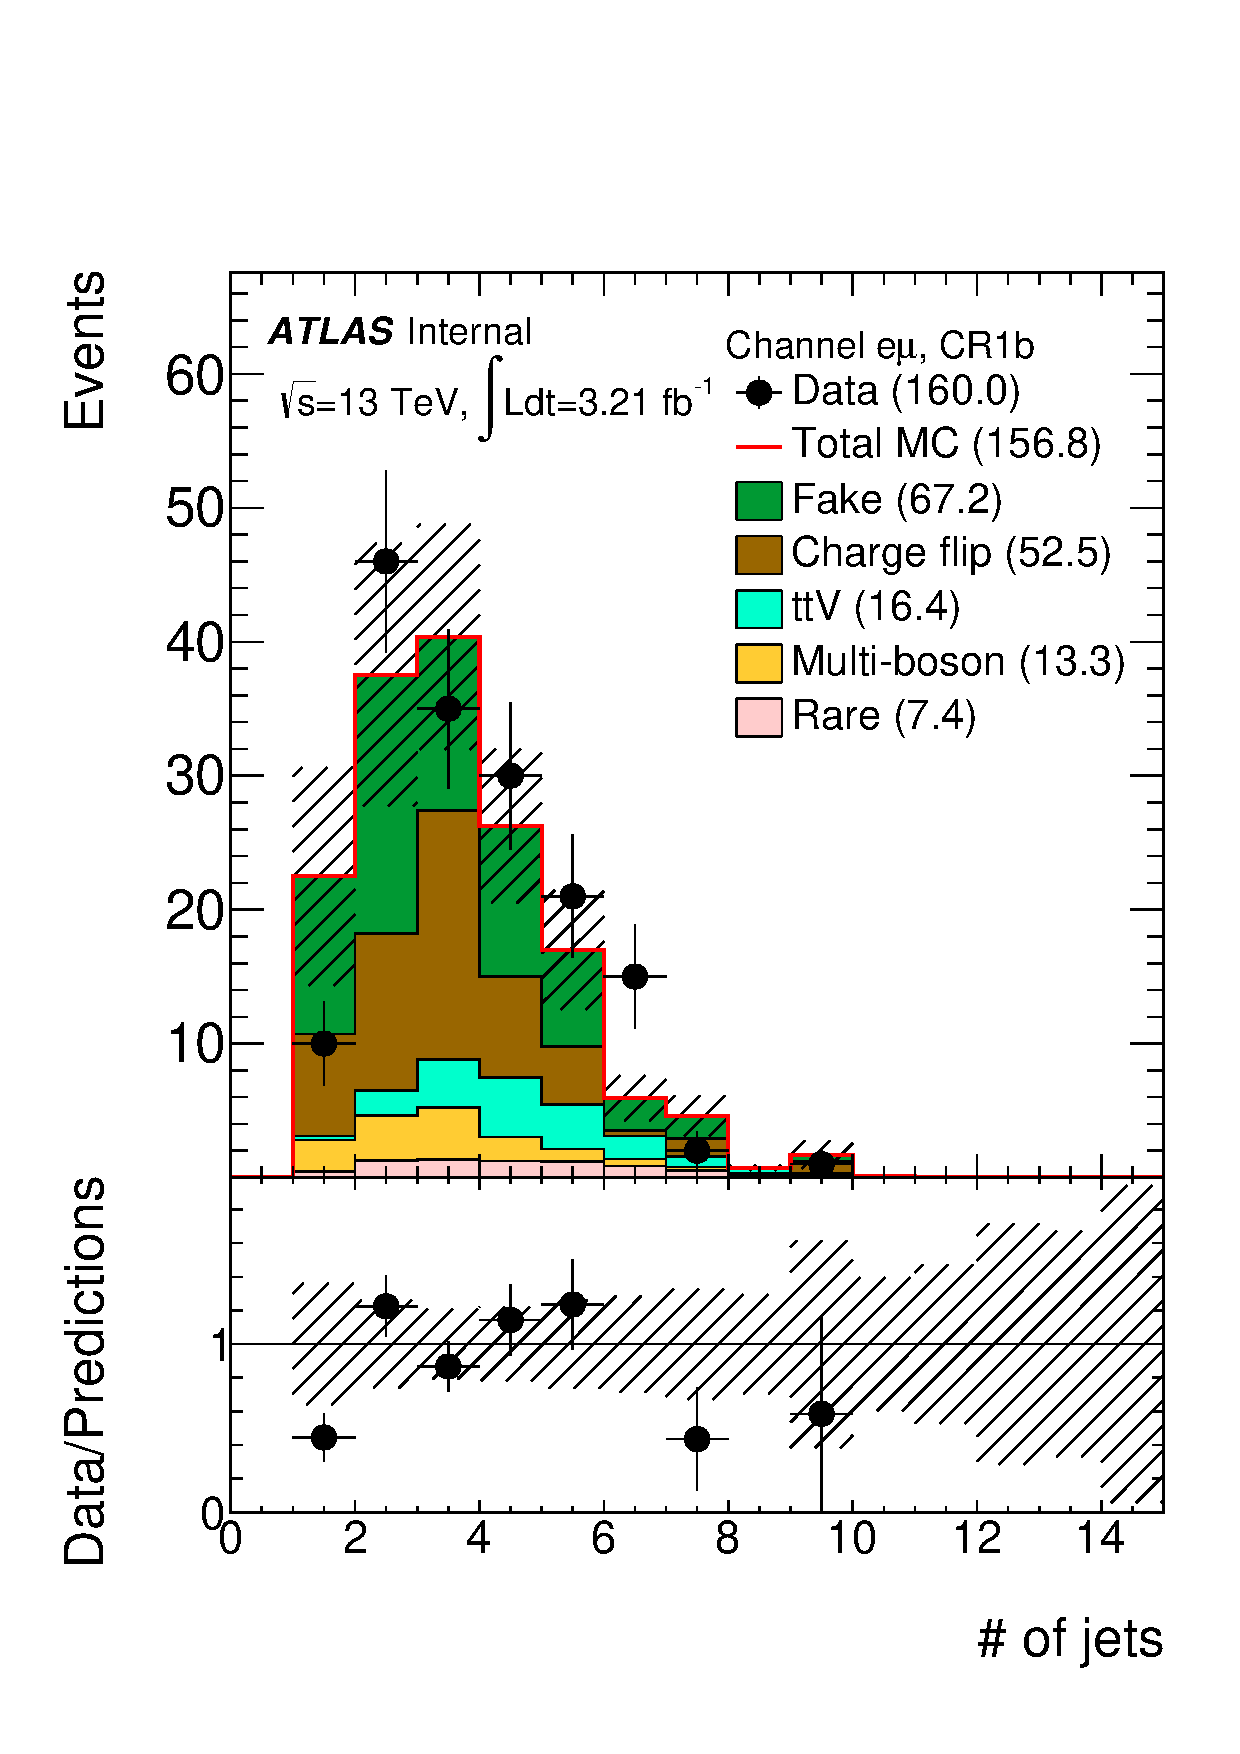
\includegraphics[width=.32\textwidth]{FIGURES/bckg_MC/SS3L/Fit/NJETS_em_CR1b_SS3L}
  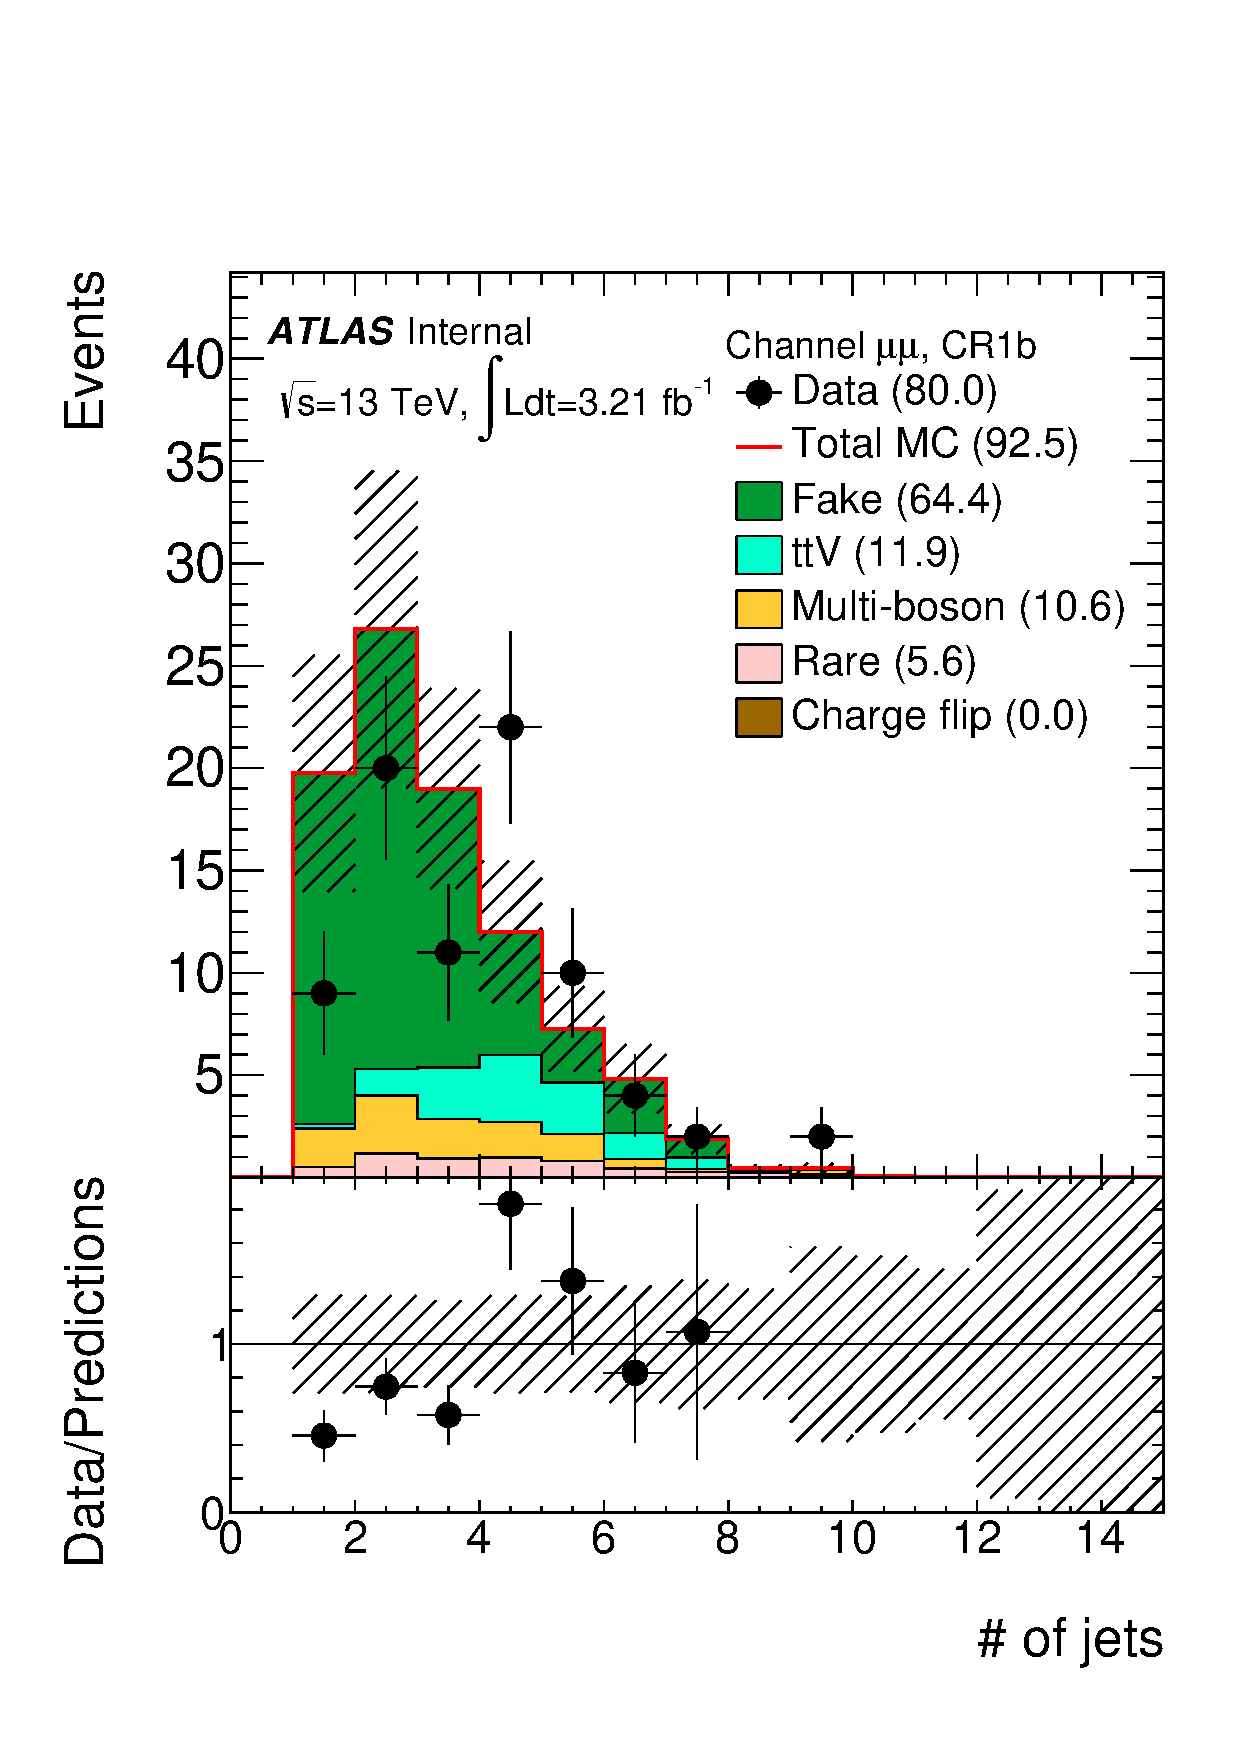
\includegraphics[width=.32\textwidth]{FIGURES/bckg_MC/SS3L/Fit/NJETS_mm_CR1b_SS3L}
\caption{
Post-fit distributions of the transverse mass for CR1b for $ee$ channel (left), $e\mu$ channel (middle), and $\mu\mu$ channel (right)  used to validate the accuracy of the simulation.
Fake-rate and charge flip corrections are applied to these distributions. The hashed band represents the sum of systematic uncertainties on the predictions.
\label{f:val_met_CR1b}
}
\end{figure}

Tables \ref{t:compare_MM_TM_VR} and  \ref{t:compare_MM_TM_SR} show the expected number of events in the validation and signal regions using the MC template method and compares it to the expectation from the nominal data-driven method to estimate the fakes and charge flip composition. The two methods are consistent within uncertainties.

  \begin{table}[htb]
    \caption{The expected number of events in the validation regions with the fake and charge flip estimations compared between the MC template method and the nominal estimates described in previous sections.
      \label{t:compare_MM_TM_VR}}
    \def\arraystretch{1.3}
    \centering

  \resizebox{\textwidth}{!}{
    \begin{tabular}{c c c c c c}
      \hline\hline
      Background & Method &  VR-WW & VR-WZ & VR-ttV & VR-ttZ \\\hline
      \hline
     Fake/non-prompt & Nominal  & $0.6 \pm 0.5$ & $8 \pm 6$ & $2.1 \pm 1.4$ & $0.6\pm 1.0$ \\
      & MC based & $0.01 \pm 0.01$ & $3.4 \pm 1.8$   & $1.8 \pm 1.0$ & $0.5 \pm 0.4$ \\
      \hline
Charge-flip & Nominal & $0.26 \pm 0.05$ & $-$ & $1.14 \pm 0.15$ & $-$  \\
      & MC based      & $< 0.08$  & $-$ & $0.27 \pm 0.23$ & $-$ \\
      \hline
    \end{tabular}}    
  \end{table}

  \begin{table}[htb]
    \caption{The expected number of events in the signal regions with the fake and charge flip estimations compared between the MC template method 
	and the nominal estimates described in previous sections. 
      \label{t:compare_MM_TM_SR}}
    \def\arraystretch{1.3}
    \centering
  \resizebox{\textwidth}{!}{
    \begin{tabular}{c c c c c c}
      \hline\hline
      Background & Method & SR0b3j & SR0b5j & SR1b & SR3b \\
      \hline
      Fake/non-prompt leptons & Nominal & $<0.2$ & $0.05\pm 0.18$ & $0.8 \pm 0.8$ & $0.13 \pm 0.17$  \\
      & MC based & $< 0.15$ & $< 0.15$  & $2.7 \pm 1.9$ & $0.02 \pm 0.01$ \\
      \hline
      Charge-flip & Nominal  & $-$ & $0.02 \pm 0.01$ & $0.60 \pm 0.12$ & $0.19 \pm 0.06$ \\
      & MC based & $-$ & $< 0.08$   & $1.0 \pm 0.8$   & $< 0.08$ \\
      \hline
    \end{tabular}}
  \end{table}


The main contributions to non-prompt leptons and charge flip events are from the high cross section processes: \ttbar, $Z$+jets, and $W$+jets. For our signal regions, the main contributor
to fakes is \ttbar. The parton showering of all these processes is done with Pythia in order to be consistent. 
The sytematic uncertainty in the method is evaluated by choosing a different generator, Sherpa. The difference in the expected number of background events due to the choice of parton shower used is taken into account in the systematic uncertainty shown in Tables \ref{t:compare_MM_TM_VR}-\ref{t:compare_MM_TM_SR}.

